% ------------------------------------------------------------------------
% Relatório Final - PIBIT 2025
% ------------------------------------------------------------------------
\documentclass[
	12pt,
	openright,
	oneside,
	a4paper,
	brazil
]{abntex2}

% ----------------------------------------------------------
% PACOTES
% ----------------------------------------------------------
\usepackage{lmodern}
\usepackage[T1]{fontenc}
\usepackage[utf8]{inputenc}
\usepackage{indentfirst}
\usepackage[dvipsnames]{xcolor}
\usepackage{graphicx}
\usepackage{microtype}
\usepackage{fancyhdr}
\usepackage[brazilian,hyperpageref]{backref}
\usepackage[alf]{abntex2cite}
\usepackage{hyperref}
\usepackage{multirow}
\usepackage{booktabs}
\usepackage{longtable}
\usepackage{array}
% Font for header (Times New Roman)
\newcommand{\headertimes}{\fontfamily{ptm}\selectfont}

% ----------------------------------------------------------
% CONFIGURAÇÕES DE PACOTES
% ----------------------------------------------------------
\renewcommand{\backrefpagesname}{Citado na(s) página(s):~}
\renewcommand{\backref}{}
\renewcommand*{\backrefalt}[4]{
	\ifcase #1 Nenhuma citação no texto.%
	\or Citado na página #2.%
	\else Citado #1 vezes nas páginas #2.%
	\fi}

% ----------------------------------------------------------
% COR UDF e CABEÇALHO INSTITUCIONAL
% ----------------------------------------------------------
\definecolor{udfblue}{HTML}{001F5F}

\pagestyle{fancy}
\fancyhf{}
\fancyfoot[C]{\thepage}
\renewcommand{\headrulewidth}{0pt}
\fancyhead[L]{%
  \raisebox{-0.5\height}{
\includegraphics[height=1.6cm]{udf.png}}%
}
\fancyhead[C]{%
  \headertimes\scriptsize\color{udfblue}%
  \begin{tabular}{c}
    \textbf{Campus Reitor Rezende Ribeiro de Rezende}\\
    SGA SUL 903, Conjunto D, Lote 79, Asa Sul\\
    70390 030 Brasília DF\\
    \textbf{T} 55 61 3704 8884
  \end{tabular}%
}
\fancyhead[R]{%
  \headertimes\scriptsize\color{udfblue}%
  \begin{tabular}{r}
    \underline{\textbf{www.udf.edu.br}}\\[4pt]
    \textbf{Campus Sede}\\
    SEP SUL EQ 704/904 Conj A\\
    70390 045 Brasília DF\\
    \textbf{T} 55 61 3704 8888
  \end{tabular}%
}
\setlength{\headheight}{2.2cm}
\setlength{\headsep}{0.5cm}

% Apply header to ALL abntex2 page styles
\fancypagestyle{plain}{%
  \fancyhf{}
  \fancyfoot[C]{\thepage}
  \renewcommand{\headrulewidth}{0pt}
  \fancyhead[L]{%
    \raisebox{-0.5\height}{
\includegraphics[height=1.6cm]{udf.png}}%
  }
  \fancyhead[C]{%
    \headertimes\scriptsize\color{udfblue}%
    \begin{tabular}{c}
      \textbf{Campus Reitor Rezende Ribeiro de Rezende}\\
      SGA SUL 903, Conjunto D, Lote 79, Asa Sul\\
      70390 030 Brasília DF\\
      \textbf{T} 55 61 3704 8884
    \end{tabular}%
  }
  \fancyhead[R]{%
    \headertimes\scriptsize\color{udfblue}%
    \begin{tabular}{r}
      \underline{\textbf{www.udf.edu.br}}\\[4pt]
      \textbf{Campus Sede}\\
      SEP SUL EQ 704/904 Conj A\\
      70390 045 Brasília DF\\
      \textbf{T} 55 61 3704 8888
    \end{tabular}%
  }
  \setlength{\headheight}{2.2cm}
}

% Override abntex2 'abntheadings' pagestyle (set by \textual)
\fancypagestyle{abntheadings}{%
  \fancyhf{}
  \fancyfoot[C]{\thepage}
  \renewcommand{\headrulewidth}{0pt}
  \fancyhead[L]{%
    \raisebox{-0.5\height}{
\includegraphics[height=1.6cm]{udf.png}}%
  }
  \fancyhead[C]{%
    \headertimes\scriptsize\color{udfblue}%
    \begin{tabular}{c}
      \textbf{Campus Reitor Rezende Ribeiro de Rezende}\\
      SGA SUL 903, Conjunto D, Lote 79, Asa Sul\\
      70390 030 Brasília DF\\
      \textbf{T} 55 61 3704 8884
    \end{tabular}%
  }
  \fancyhead[R]{%
    \headertimes\scriptsize\color{udfblue}%
    \begin{tabular}{r}
      \underline{\textbf{www.udf.edu.br}}\\[4pt]
      \textbf{Campus Sede}\\
      SEP SUL EQ 704/904 Conj A\\
      70390 045 Brasília DF\\
      \textbf{T} 55 61 3704 8888
    \end{tabular}%
  }
  \setlength{\headheight}{2.2cm}
}

% ---
% Informações para CAPA e FOLHA DE ROSTO
% ---
\titulo{Relatório Final\\Desenvolvimento de um Dashboard para o Monitoramento e Acompanhamento Contínuo de Projetos em Fábricas de Software Acadêmicas}
\autor{Danrley Willyan da Silva Pereira (RGM 42570166)}
\orientador{Prof.ª Kerlla de Souza Luz}
\local{Brasília}
\data{2026}
\instituicao{
  Centro Universitário do Distrito Federal (UDF)\\
  Programa Institucional de Bolsas de Iniciação em Desenvolvimento Tecnológico e Inovação (PIBIT)
}

% ---
% Configurações de hyperref
% ---
\makeatletter
\hypersetup{
	pdftitle={\@title},
	pdfauthor={\@author},
	pdfsubject={Relatório Final PIBIT},
	pdfkeywords={Dashboard, Fábrica de Software Acadêmica, Métricas, KPIs, Arquitetura Medalhão, D3.js},
	colorlinks=true,
	linkcolor=blue,
	citecolor=blue,
	filecolor=magenta,
	urlcolor=blue,
}
\makeatother

% Espaçamento
\setlength{\parindent}{1.3cm}
\setlength{\parskip}{0.2cm}

% Margem inferior maior para evitar conteúdo colado ao final da página
\setlength{\textheight}{\textheight}
\addtolength{\textheight}{-1.5cm}

\makeindex

% ----
% Início do documento
% ----
\begin{document}
\selectlanguage{brazil}
\frenchspacing

% Forçar cabeçalho institucional em todas as páginas
\pagestyle{fancy}

% ----------------------------------------------------------
% ELEMENTOS TEXTUAIS
% ----------------------------------------------------------
\textual
\pagestyle{fancy}

% ===============================
% RELATÓRIO FINAL (PIBIT/2025-2026)
% ===============================

% ----------------------------------------------------------
% 1. IDENTIFICAÇÃO DO PROJETO
% ----------------------------------------------------------
\section*{1.\ Identificação do Projeto}

\begin{tabular}{|p{4.5cm}|p{10cm}|}
\hline
\textbf{Aluno Pesquisador:} & Esp.\ Danrley Pereira \\
\hline
\textbf{Orientador:} & Dra.\ Kerlla de Souza Luz \\
\hline
\textbf{Área de conhecimento do Projeto:} &
Ciências Exatas e da Terra \newline
\hspace*{0.5em}» Ciência da Computação \newline
\hspace*{1.0em}» » Metodologia e Técnicas da Computação \newline
\hspace*{1.5em}» » » Engenharia de Software \\
\hline
\textbf{Título do Projeto:} &
Desenvolvimento de um Dashboard para o Monitoramento e Acompanhamento Contínuo de Projetos em Fábricas de Software Acadêmicas \\
\hline
\end{tabular}

% ----------------------------------------------------------
% 2. RESUMO
% ----------------------------------------------------------
\section*{2.\ Resumo}

Este relatório final apresenta os resultados completos do projeto PIBIT que desenvolveu o \textbf{Dashboard de Monitoramento de Métricas de Produtividade e Qualidade} --- uma plataforma \textit{open source} para monitoramento de projetos em fábricas de software acadêmicas. O projeto, que teve início com uma revisão de literatura e definição de KPIs (relatório parcial, set/2025), evoluiu para uma aplicação \textit{full-stack} em produção, co-desenvolvida em colaboração com a \textbf{Dra.\ Carla Rocha} (professora de Métodos de Desenvolvimento de Software --- MDS, na Universidade de Brasília). A plataforma implementa integralmente a \textbf{Arquitetura Medalhão} (Bronze$\rightarrow$Silver$\rightarrow$Gold), conta com \textbf{13+ páginas interativas} com visualizações D3.js, análise por inteligência artificial via API Google Gemini e duas instâncias em produção: \textbf{UnB} (\url{https://unb-mds.github.io/2025-2-Squad-01/}) e \textbf{UDF/LabTech} (\url{https://labtechudf.github.io/CoOps/}). Danrley construiu a plataforma e iterou diretamente com Dra.\ Carla para definir quais dados Silver e Gold ela necessitava para suas disciplinas. Ao final do semestre, Dra.\ Carla utilizou o dashboard para avaliar seus alunos --- validando o software em contexto pedagógico real. A otimização do pipeline de extração alcançou ganho de \textbf{100x} em desempenho. O frontend atinge \textbf{94\% de cobertura de testes}. O dashboard é distribuído sob licença \textbf{GPL v3.0} e opera com \textbf{infraestrutura zero} via GitHub Pages e GitHub Actions.

% ----------------------------------------------------------
% 3. INTRODUÇÃO
% ----------------------------------------------------------
\section*{3.\ Introdução}

As fábricas de software acadêmicas desempenham papel fundamental na formação de profissionais de tecnologia, oferecendo aos estudantes experiências práticas com projetos reais e metodologias ágeis \cite{dos2021experiencia,romanha2016modelo,fernandes2004fabrica}. Contudo, a gestão e o monitoramento dessas equipes é um desafio persistente: docentes e coordenadores precisam acompanhar o progresso, identificar gargalos e avaliar contribuições individuais em um contexto onde dezenas de repositórios e equipes operam simultaneamente \cite{hamer2021using,barbosaIndicadoresConjunto2016}.

A proposta original deste projeto PIBIT visava desenvolver um \textit{dashboard} para monitoramento contínuo de projetos em fábricas de software acadêmicas, com coleta de dados via API do GitHub e visualização de KPIs técnicos e colaborativos. O relatório parcial (setembro de 2025) documentou a revisão de literatura, a definição do conjunto inicial de KPIs e os protótipos iniciais --- um script Python de extração e um Jupyter notebook com 20 visualizações estáticas.

Após o relatório parcial, o projeto evoluiu significativamente em escopo e maturidade. A fábrica de software LabTech do UDF não possuía projeto ativo no segundo semestre de 2025, o que motivou a busca por uma colaboração externa. A parceria foi estabelecida com a \textbf{Dra.\ Carla Rocha}, professora de Métodos de Desenvolvimento de Software (MDS) na Universidade de Brasília (UnB), que já havia sido entrevistada na fase de levantamento qualitativo (Apêndice A). Dra.\ Carla coordena disciplinas nas quais dezenas de equipes de estudantes desenvolvem projetos de software em organizações GitHub, configurando um cenário ideal para validação da plataforma.

A partir dessa colaboração, os protótipos iniciais deram lugar ao \textbf{Dashboard de Monitoramento de Métricas de Produtividade e Qualidade} --- uma plataforma \textit{full-stack} de código aberto para análise cooperativa de organizações GitHub. Danrley construiu a plataforma e colaborou diretamente com Dra.\ Carla para decidir quais dados das camadas Silver e Gold ela necessitava para acompanhar e avaliar suas turmas. O processo foi iterativo: juntos, eles definiram métricas, visualizações e camadas de dados. Um módulo de análise por inteligência artificial foi adicionado para gerar resumos em linguagem natural das contribuições dos membros.

A validação mais significativa ocorreu ao final do semestre, quando Dra.\ Carla utilizou o dashboard para \textbf{avaliar seus alunos} --- demonstrando que o software atende a necessidades reais de avaliação pedagógica em fábricas de software acadêmicas.

O dashboard tem relevância tanto para a \textbf{academia} --- ao possibilitar avaliação baseada em evidências de equipes de software --- quanto para a \textbf{indústria} --- ao fornecer um pipeline de analytics reproduzível, de custo zero e aplicável a qualquer organização GitHub \cite{kitchenham2010s,ozkan2019agile}.

% ----------------------------------------------------------
% 4. MATERIAIS E MÉTODOS
% ----------------------------------------------------------
\section*{4.\ Materiais e Métodos}

\subsection*{4.1 Abordagem metodológica}

O projeto adotou abordagem de \textbf{métodos mistos} (quanti-qualitativa). A componente qualitativa envolveu entrevistas semiestruturadas com gestores de fábricas de software acadêmicas (Apêndice A --- LAPPIS/UnB; Apêndice B --- LabTech/UDF), que orientaram o desenho dos KPIs e a priorização de funcionalidades. A componente quantitativa se materializou na extração automatizada de dados via API do GitHub e na produção de métricas e visualizações para análise de equipes.

O desenvolvimento seguiu ciclos iterativos de co-desenvolvimento: Danrley construía funcionalidades no dashboard, apresentava os resultados a Dra.\ Carla Rocha (UnB), e ambos decidiam conjuntamente os próximos dados e visualizações a serem incorporados nas camadas Silver e Gold. Esse modelo de co-desenvolvimento academia-academia é sustentado pela literatura sobre colaboração e co-criação \cite{bjerregaard2021lessons,jarvela2018collaboration,franssen2019cogs}.

\subsection*{4.2 Pipeline de dados: Arquitetura Medalhão}

A extração de dados utiliza uma abordagem híbrida \textbf{REST API + GraphQL} do GitHub, organizada na Arquitetura Medalhão em três camadas:

\begin{itemize}
    \item \textbf{Bronze (ingestão)}: 7 módulos de extração --- repositórios, membros, issues, commits, pull requests, eventos e estrutura de repositórios. Dados armazenados em formato JSON com linhagem preservada.
    \item \textbf{Silver (processamento)}: 6 módulos de transformação --- analytics de membros, métricas de contribuição, redes de colaboração, análise temporal, estatísticas de membros e análise de arquivos/linguagens.
    \item \textbf{Gold (consumo)}: KPIs executivos para o dashboard, agregação temporal e classificação de desempenho.
\end{itemize}

As Figuras~\ref{fig:dag-medalhao} e \ref{fig:sequencia-etl} (Apêndice~\ref{apendiceD}) detalham o fluxo do pipeline e o processo ETL automatizado.

\subsection*{4.3 Stack tecnológico}

\begin{itemize}
    \item \textbf{Backend}: Python (extração, transformação, análise por IA)
    \item \textbf{Frontend}: React 19, TypeScript, D3.js, Vite, Tailwind CSS
    \item \textbf{CI/CD}: GitHub Actions (pipeline diário às 5h UTC)
    \item \textbf{Hospedagem}: GitHub Pages (infraestrutura zero)
    \item \textbf{IA}: API Google Gemini para análise em linguagem natural
    \item \textbf{Licença}: GPL v3.0
\end{itemize}

\subsection*{4.4 Testes e qualidade}

\begin{itemize}
    \item \textbf{Frontend}: Vitest + React Testing Library, com \textbf{94\% de cobertura}
    \item \textbf{Backend}: pytest para testes unitários e de integração
    \item \textbf{CI/CD}: execução automática de testes a cada push e no pipeline diário
\end{itemize}

\subsection*{4.5 Dados qualitativos}

Entrevistas semiestruturadas foram conduzidas em dois contextos institucionais:
\begin{itemize}
    \item \textbf{Apêndice A}: Entrevista com Dra.\ Carla Rocha (LAPPIS/UnB --- FGA), que validou a abordagem da Arquitetura Medalhão, a periodicidade semanal e a importância de grafos de rede para identificação de perfis de colaboração.
    \item \textbf{Apêndice B}: Relatos da fábrica LabTech/UDF, que contribuíram com indicadores de adesão inicial (clones, inclinação nas primeiras 8 semanas) e distinção de papéis (integrador vs.\ especialista).
\end{itemize}

Cada imagem (tabelas, gráficos, figuras) é citada no texto e apresentada nos Apêndices com respectiva identificação.

% ----------------------------------------------------------
% 5. RESULTADOS FINAIS
% ----------------------------------------------------------
\section*{5.\ Resultados Finais}

\subsection*{5.1 Visão geral da plataforma}

O dashboard é uma aplicação \textit{full-stack} de código aberto para análise cooperativa de organizações GitHub. A plataforma transforma dados brutos de repositórios em insights acionáveis por meio de visualizações interativas e análise por inteligência artificial. Duas instâncias estão em produção:

\begin{itemize}
    \item \textbf{UnB (MDS)}: \url{https://unb-mds.github.io/2025-2-Squad-01/} --- analisa a organização \texttt{unb-mds} com 70+ repositórios de equipes de alunos.
    \item \textbf{UDF (LabTech)}: \url{https://labtechudf.github.io/CoOps/} --- analisa a organização \texttt{LabTechUDF}.
\end{itemize}

\begin{figure}[ht]
\centering
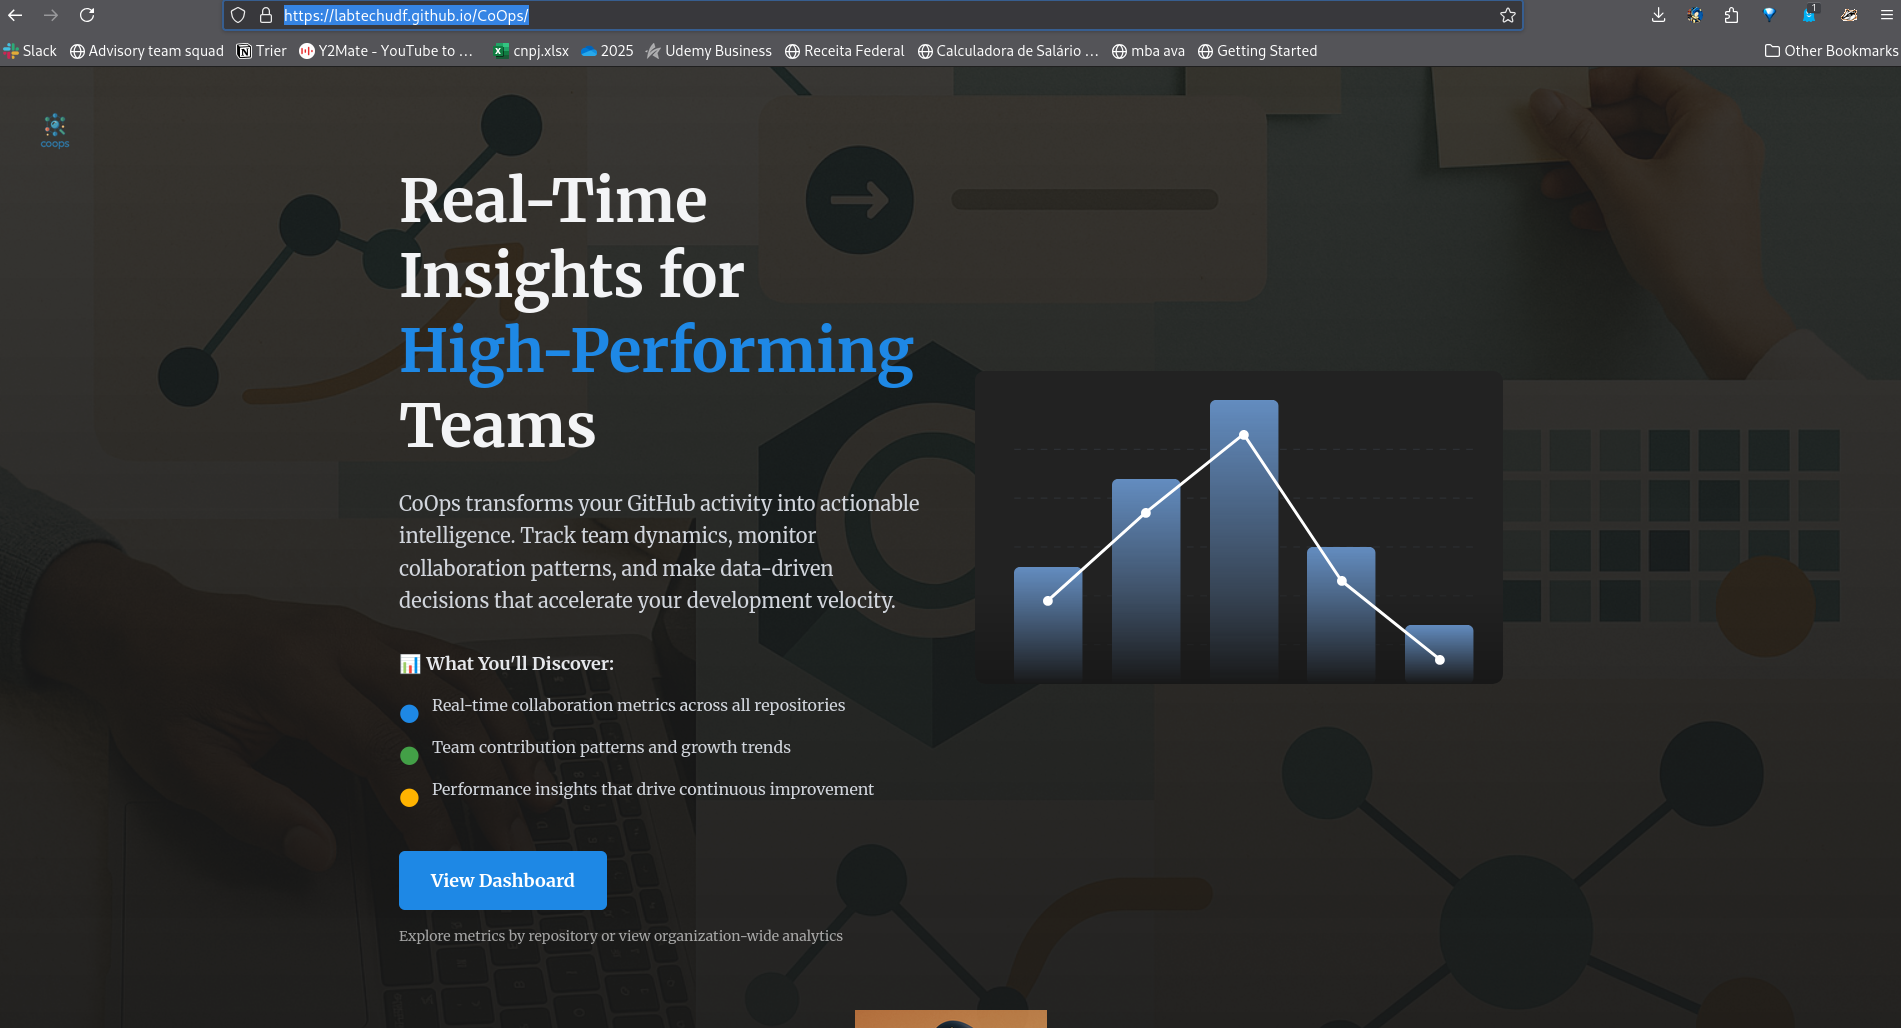
\includegraphics[width=0.9\textwidth]{screenshot-coops/pagina-inicial.png}
\caption{Página inicial do dashboard (\url{https://labtechudf.github.io/CoOps/}), exibindo a visão geral da organização com navegação para repositórios, membros e visualizações.}
\label{fig:pagina-inicial}
\end{figure}

\subsection*{5.2 Pipeline de dados (Arquitetura Medalhão)}

O pipeline implementa integralmente a Arquitetura Medalhão:

\textbf{Camada Bronze} --- 7 módulos de extração:
\begin{enumerate}
    \item Repositórios (metadados, linguagens, tópicos)
    \item Membros (perfis, permissões)
    \item Issues (estados, atribuições, comentários)
    \item Commits (autores, timestamps, diffs)
    \item Pull requests (revisões, comentários, merge status)
    \item Eventos (timeline de atividades)
    \item Estrutura de repositórios (árvore de arquivos, linguagens por arquivo)
\end{enumerate}

\textbf{Camada Silver} --- 6 módulos de processamento:
\begin{enumerate}
    \item Analytics de membros (contribuições agregadas por tipo)
    \item Métricas de contribuição (code churn, frequência, distribuição)
    \item Redes de colaboração (grafos autor$\leftrightarrow$revisor)
    \item Análise temporal (séries por semana, tendências)
    \item Estatísticas de membros (classificação de desempenho)
    \item Análise de arquivos e linguagens (distribuição, diversidade)
\end{enumerate}

\textbf{Camada Gold} --- Agregações executivas:
\begin{itemize}
    \item KPIs por repositório e por organização
    \item Timeline agregada para visualização de tendências
    \item Classificação de membros em tiers de desempenho
\end{itemize}

\textbf{Otimização de desempenho}: a migração de chamadas GraphQL para REST API resultou em ganho de \textbf{100x} no tempo de extração (de 3--4 horas para 30--40 segundos por organização), viabilizando a execução diária automatizada.

\begin{figure}[ht]
\centering
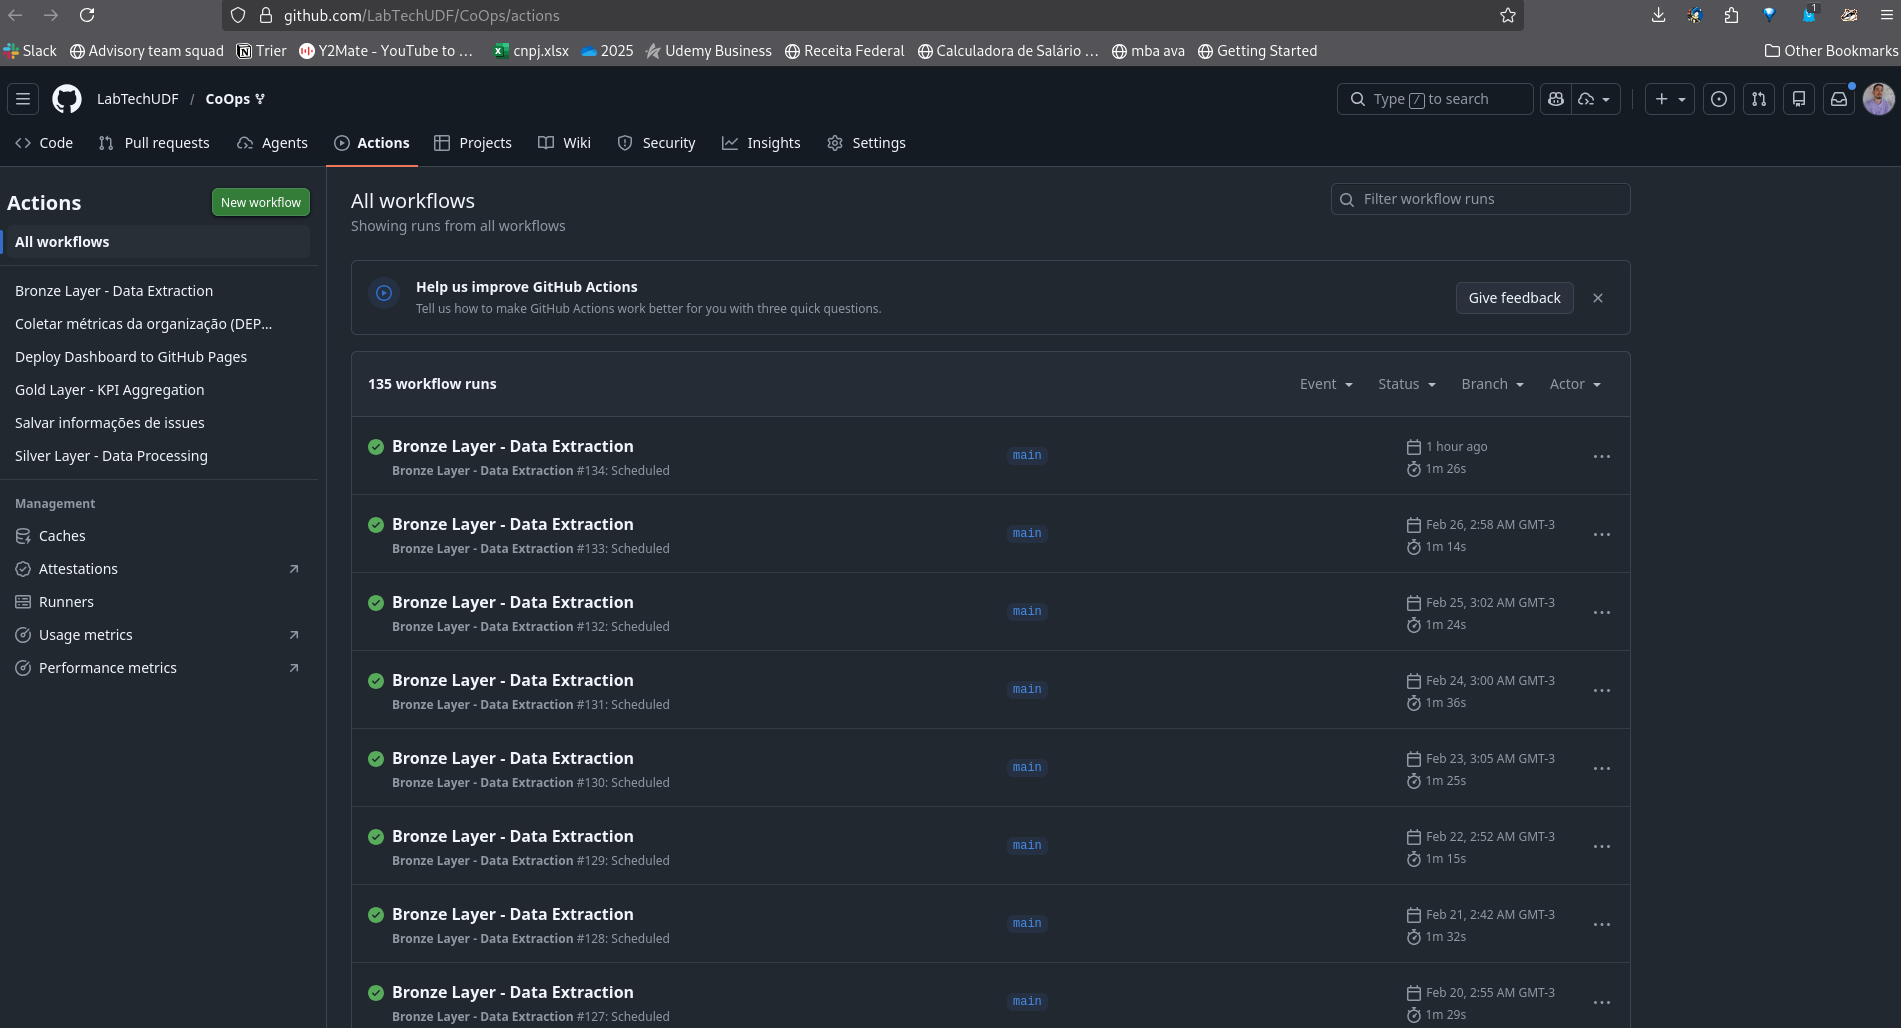
\includegraphics[width=0.9\textwidth]{screenshot-coops/pipelines-github-todos-workflows-rodados.png}
\caption{Workflows do GitHub Actions executando o pipeline de extração e transformação de dados do dashboard. Cada execução processa as camadas Bronze, Silver e Gold automaticamente.}
\label{fig:pipeline-github}
\end{figure}

\begin{figure}[ht]
\centering
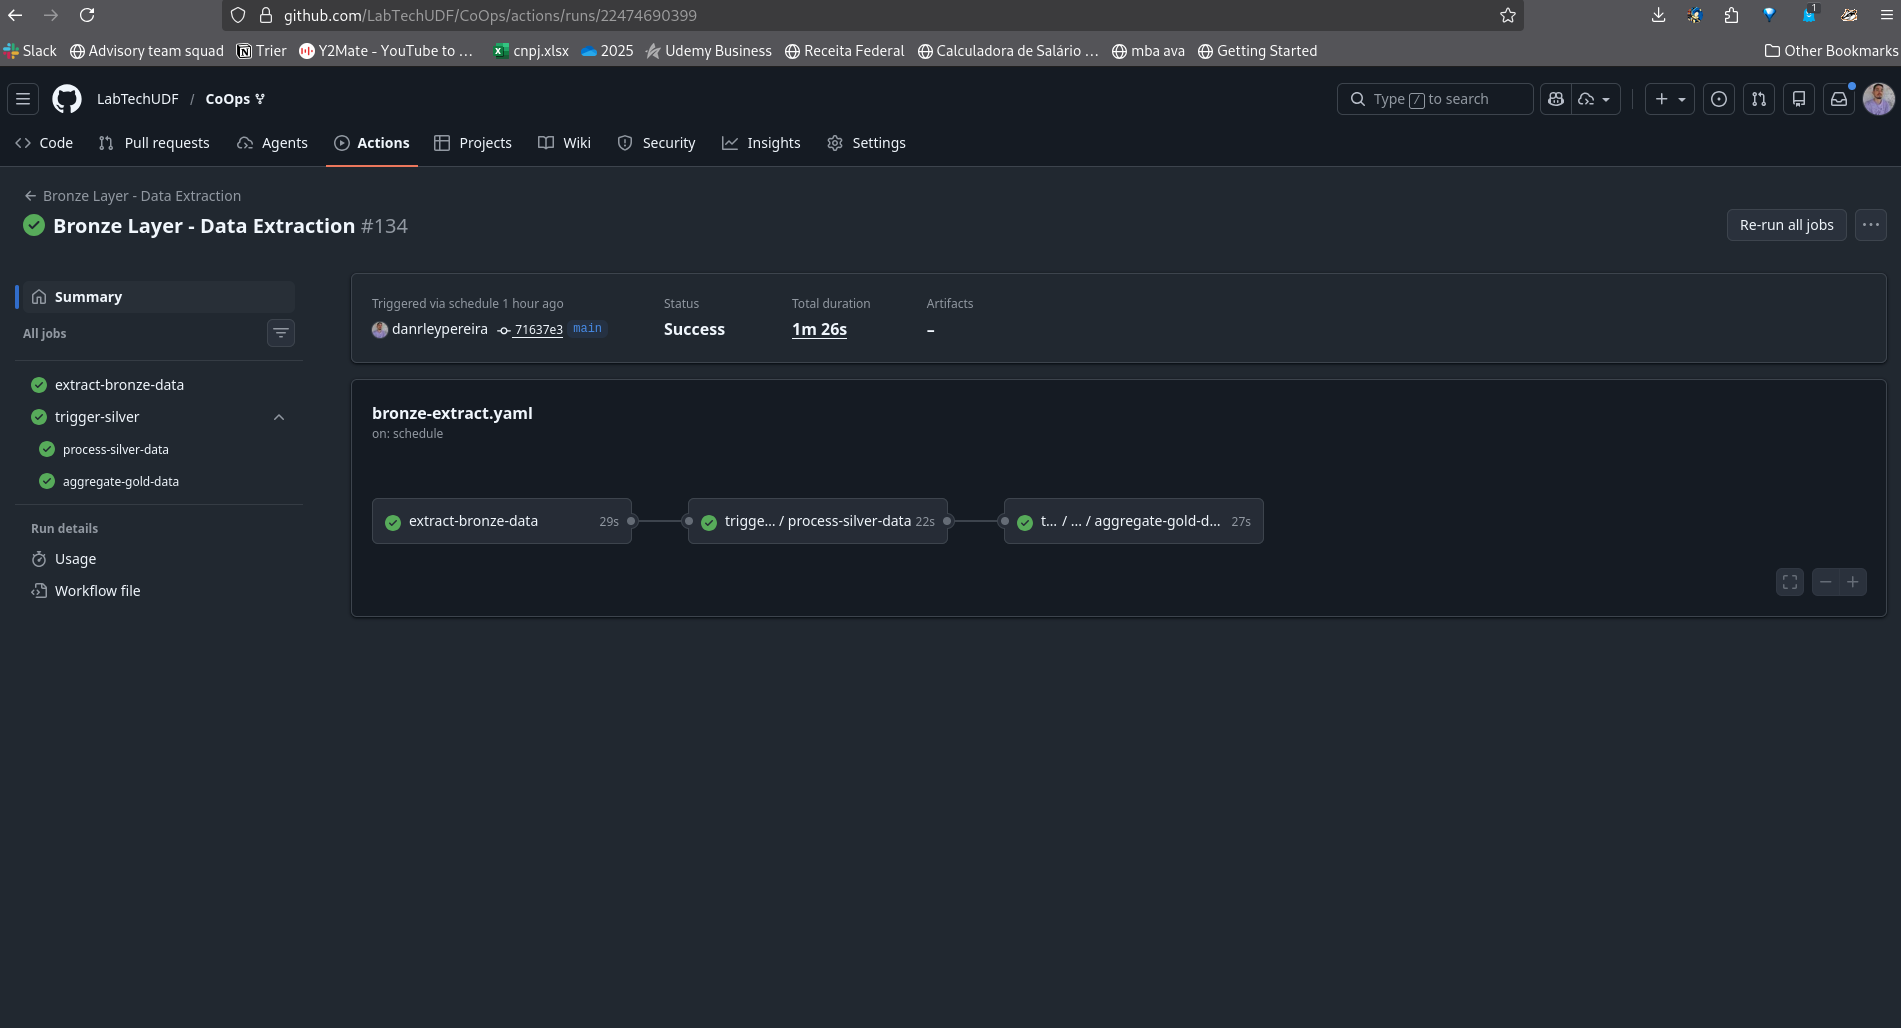
\includegraphics[width=0.9\textwidth]{screenshot-coops/pipelines-github-bronze.png}
\caption{Detalhe da execução do pipeline Bronze no GitHub Actions, mostrando os módulos de extração de dados da API do GitHub.}
\label{fig:pipeline-bronze}
\end{figure}

\subsection*{5.3 Frontend: dashboard e visualizações}

O frontend conta com \textbf{13+ páginas interativas} construídas com React 19 e D3.js. As principais visualizações incluem:

\begin{itemize}
    \item \textbf{Treemap}: distribuição de repositórios por tamanho, atividade ou linguagem
    \item \textbf{CirclePack}: hierarquia de contribuições por membro e repositório
    \item \textbf{Rede de colaboração}: grafo interativo de interações entre membros (commits, issues, PRs)
    \item \textbf{Activity Heatmap}: padrões temporais de atividade (dia da semana $\times$ hora)
    \item \textbf{Timeline}: evolução temporal de métricas por repositório
    \item \textbf{Fingerprint de repositório}: análise de composição e estrutura de arquivos
    \item \textbf{Análise de commits}: frequência, distribuição e padrões por autor
    \item \textbf{Métricas de issues/PRs}: throughput, lead time, participação em revisões
    \item \textbf{KPIs executivos}: visão consolidada da organização com indicadores-chave
\end{itemize}

\begin{figure}[ht]
\centering
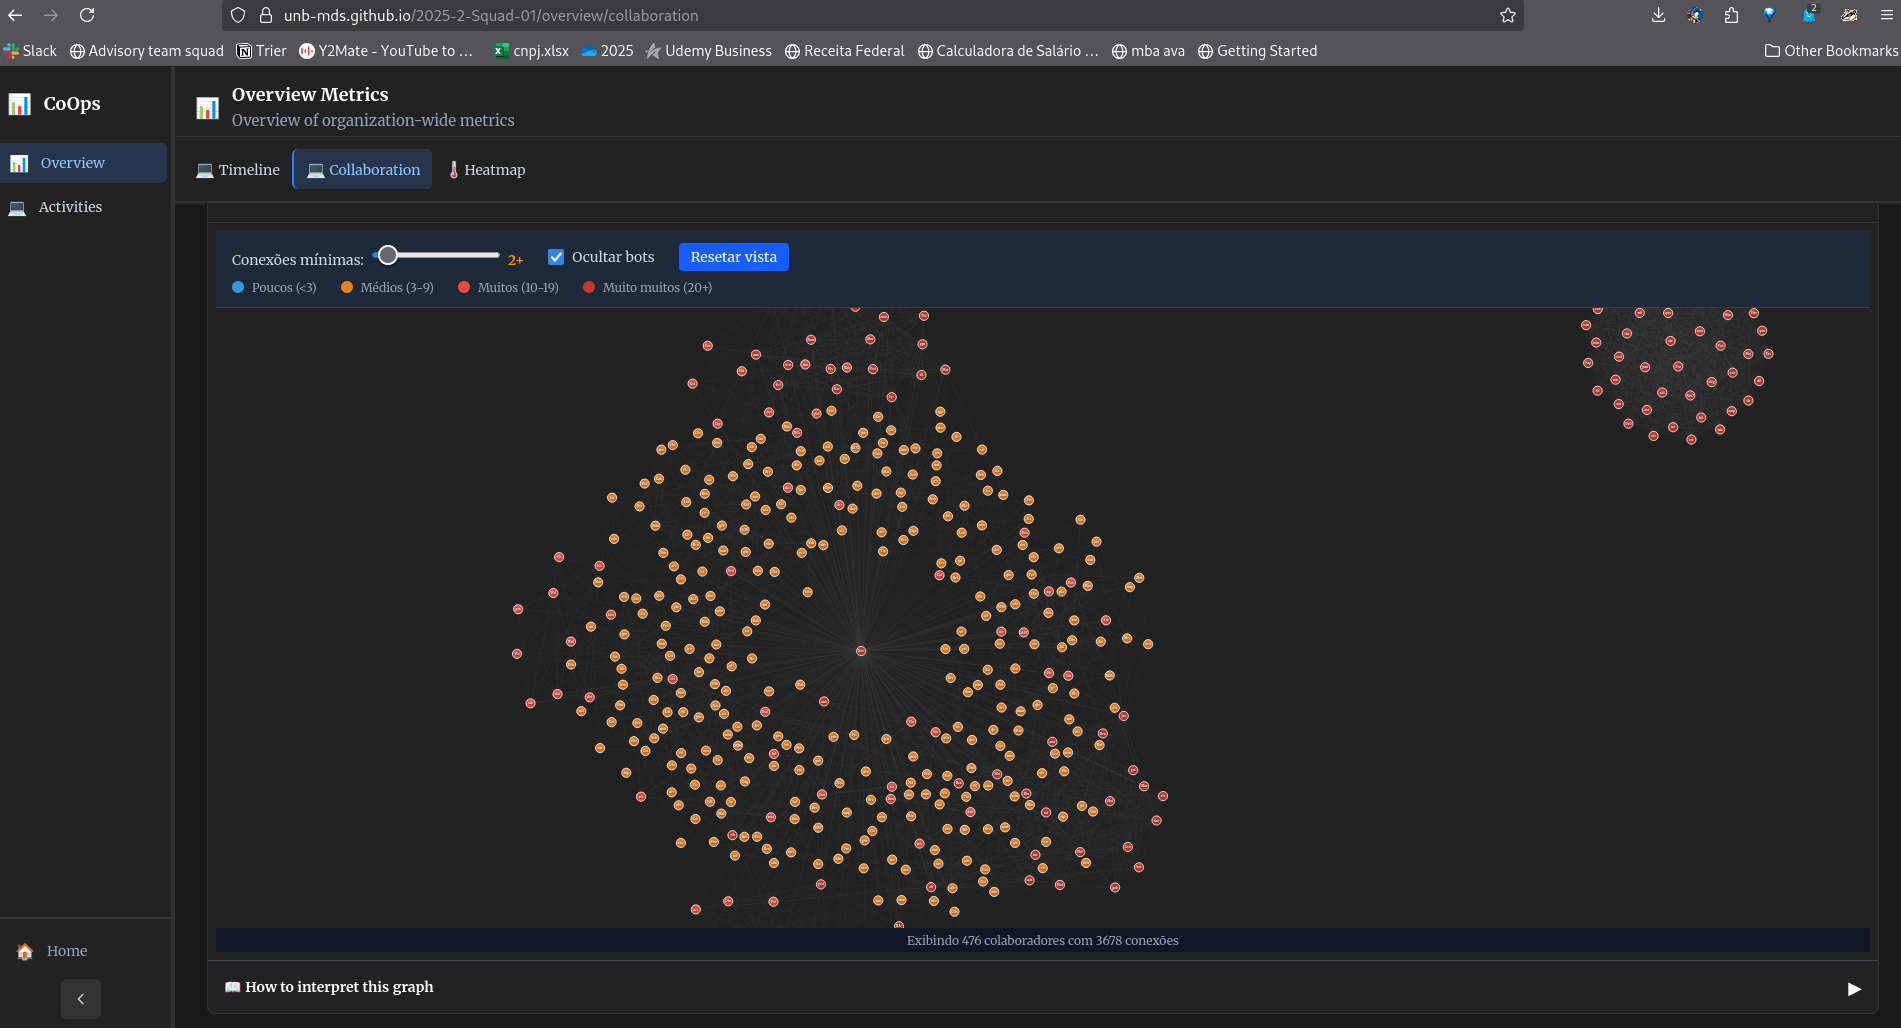
\includegraphics[width=0.9\textwidth]{screenshot-coops/rede-de-colaboracao.png}
\caption{Rede de colaboração interativa construída com D3.js. O grafo exibe as interações entre membros da organização, permitindo identificar \textit{hubs} de colaboração e padrões de conectividade.}
\label{fig:rede-colaboracao-coops}
\end{figure}

\begin{figure}[ht]
\centering
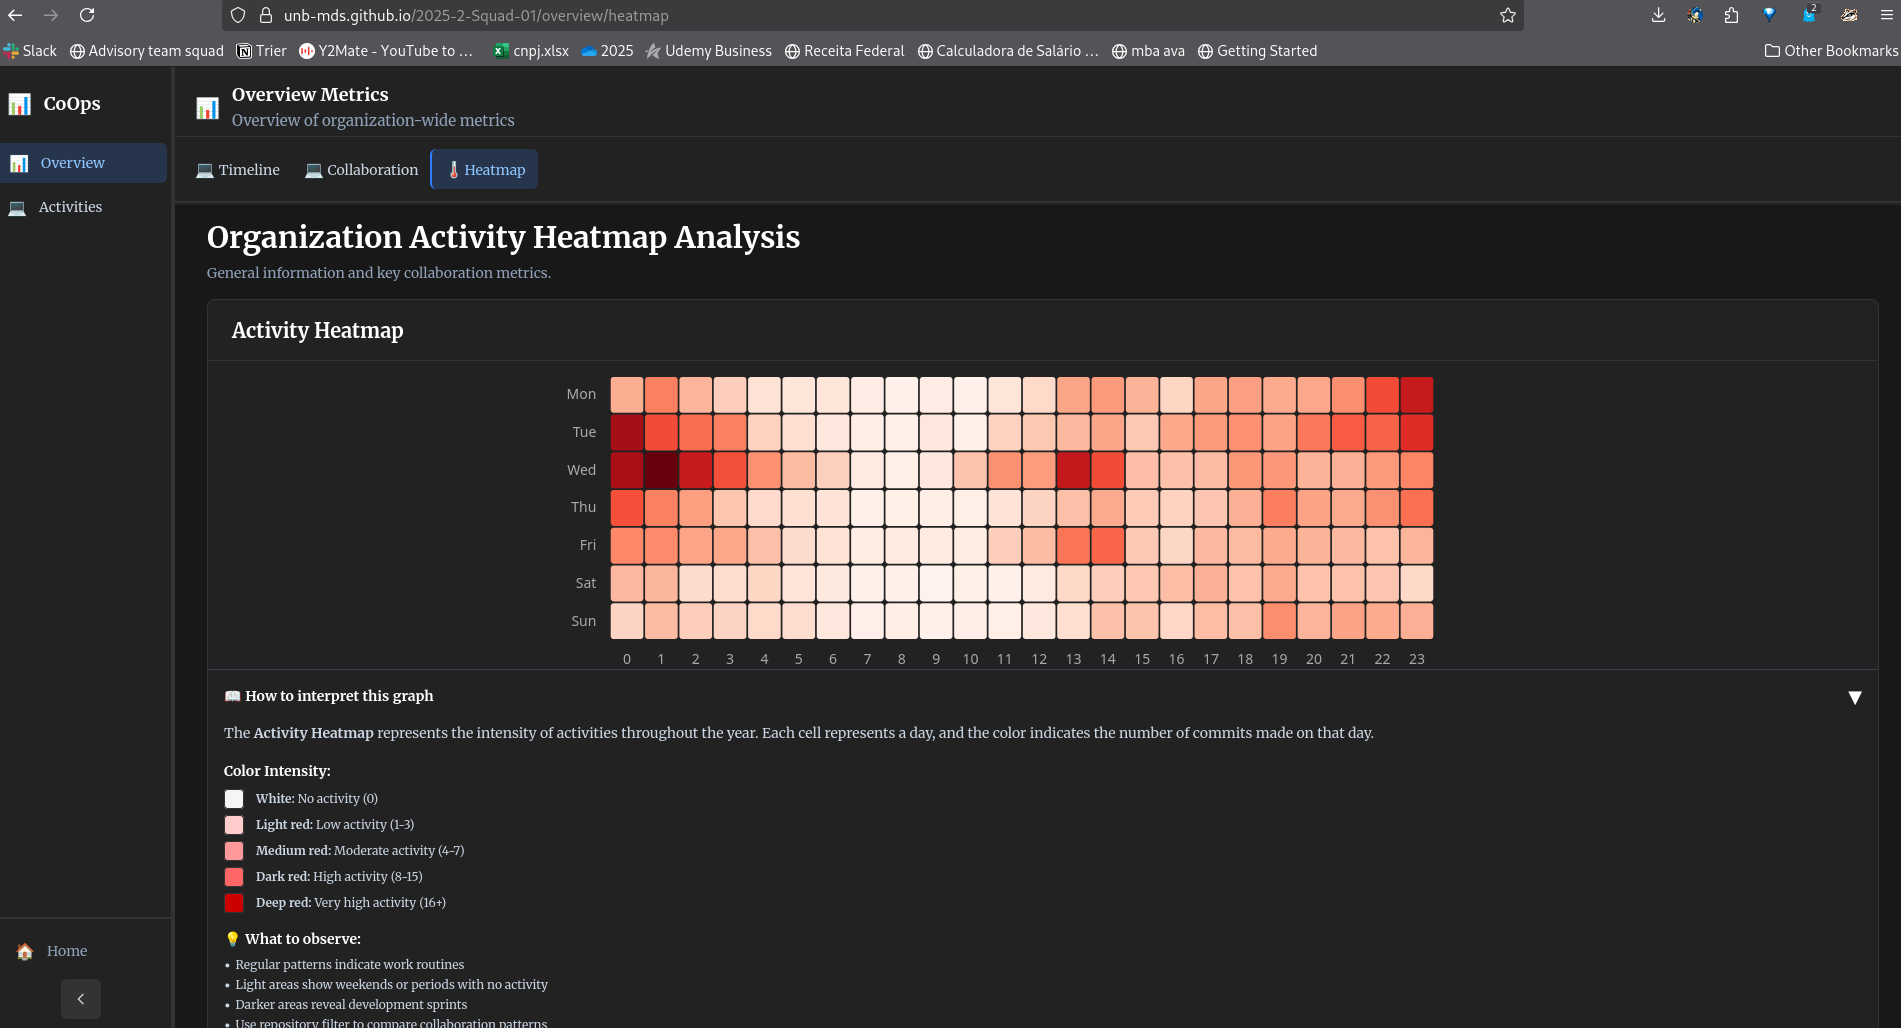
\includegraphics[width=0.9\textwidth]{screenshot-coops/heatmap.png}
\caption{Heatmap de atividade do dashboard, exibindo padrões temporais de contribuições (dia da semana $\times$ hora do dia).}
\label{fig:heatmap-coops}
\end{figure}

\begin{figure}[ht]
\centering
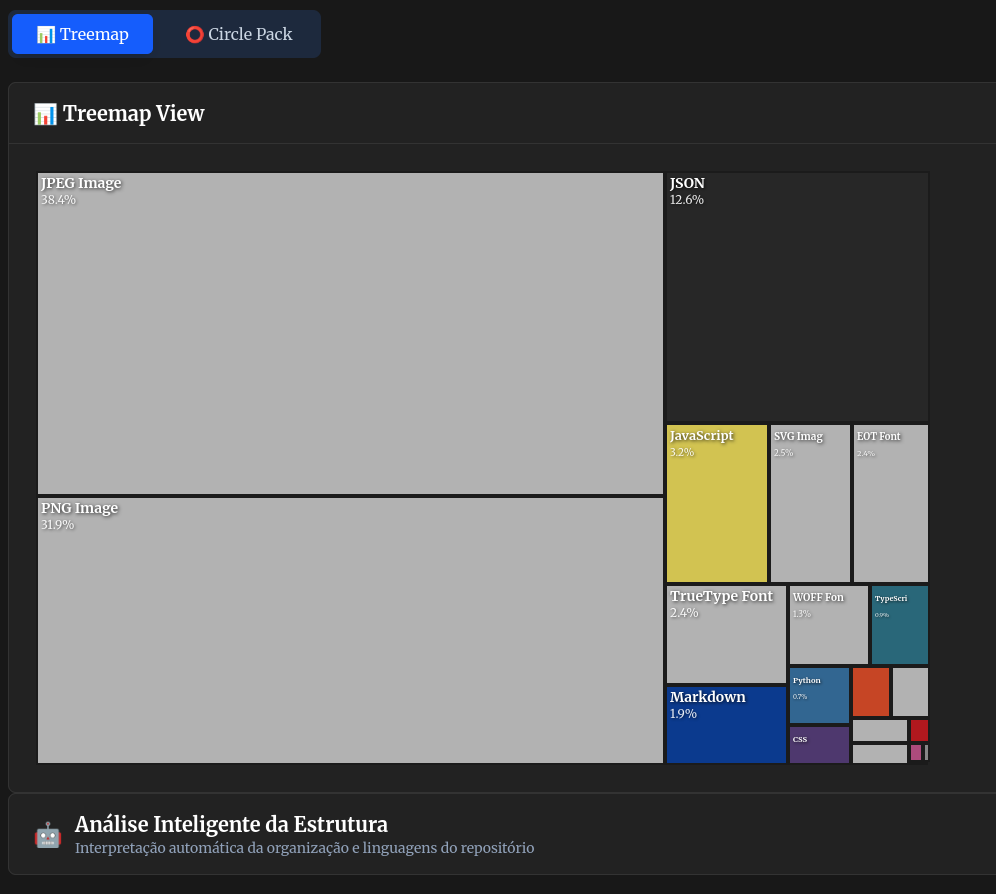
\includegraphics[width=0.9\textwidth]{screenshot-coops/treemap.png}
\caption{Visualização treemap dos repositórios da organização, onde o tamanho de cada bloco representa o volume de atividade.}
\label{fig:treemap-coops}
\end{figure}

\begin{figure}[ht]
\centering
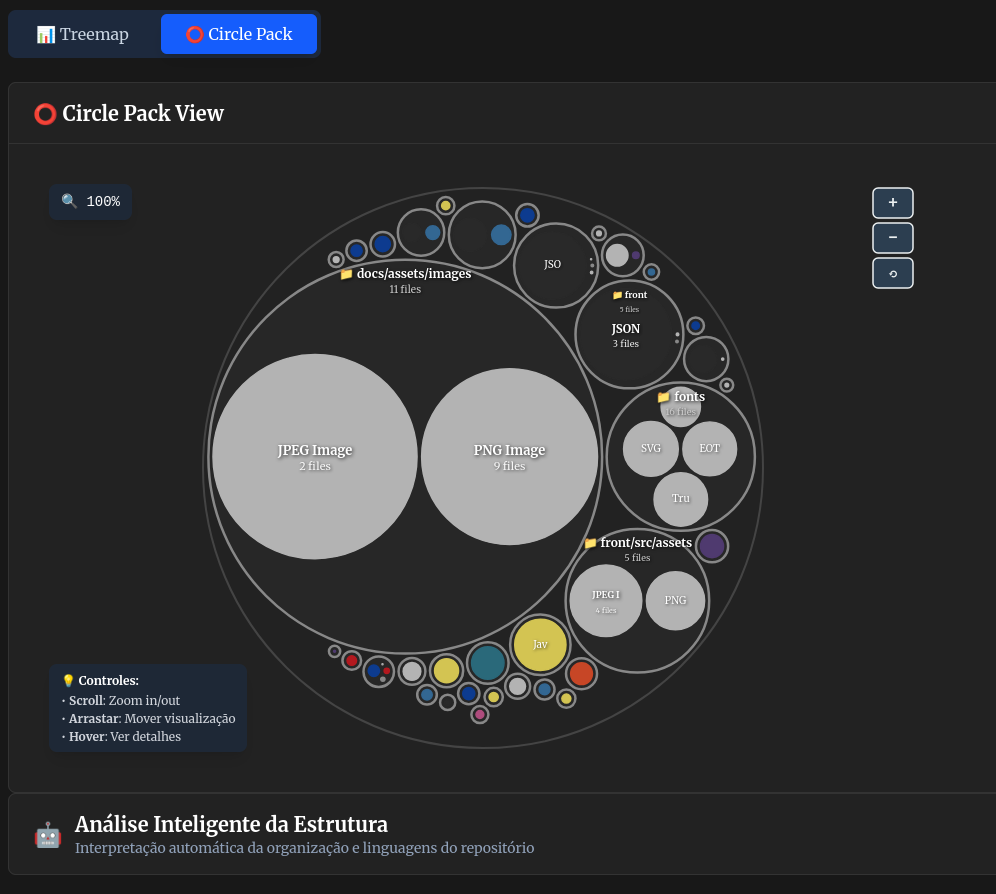
\includegraphics[width=0.9\textwidth]{screenshot-coops/circlepack-view.png}
\caption{Visualização CirclePack hierárquica de contribuições por membro e repositório, permitindo navegação interativa entre níveis de agregação.}
\label{fig:circlepack-coops}
\end{figure}

\begin{figure}[ht]
\centering
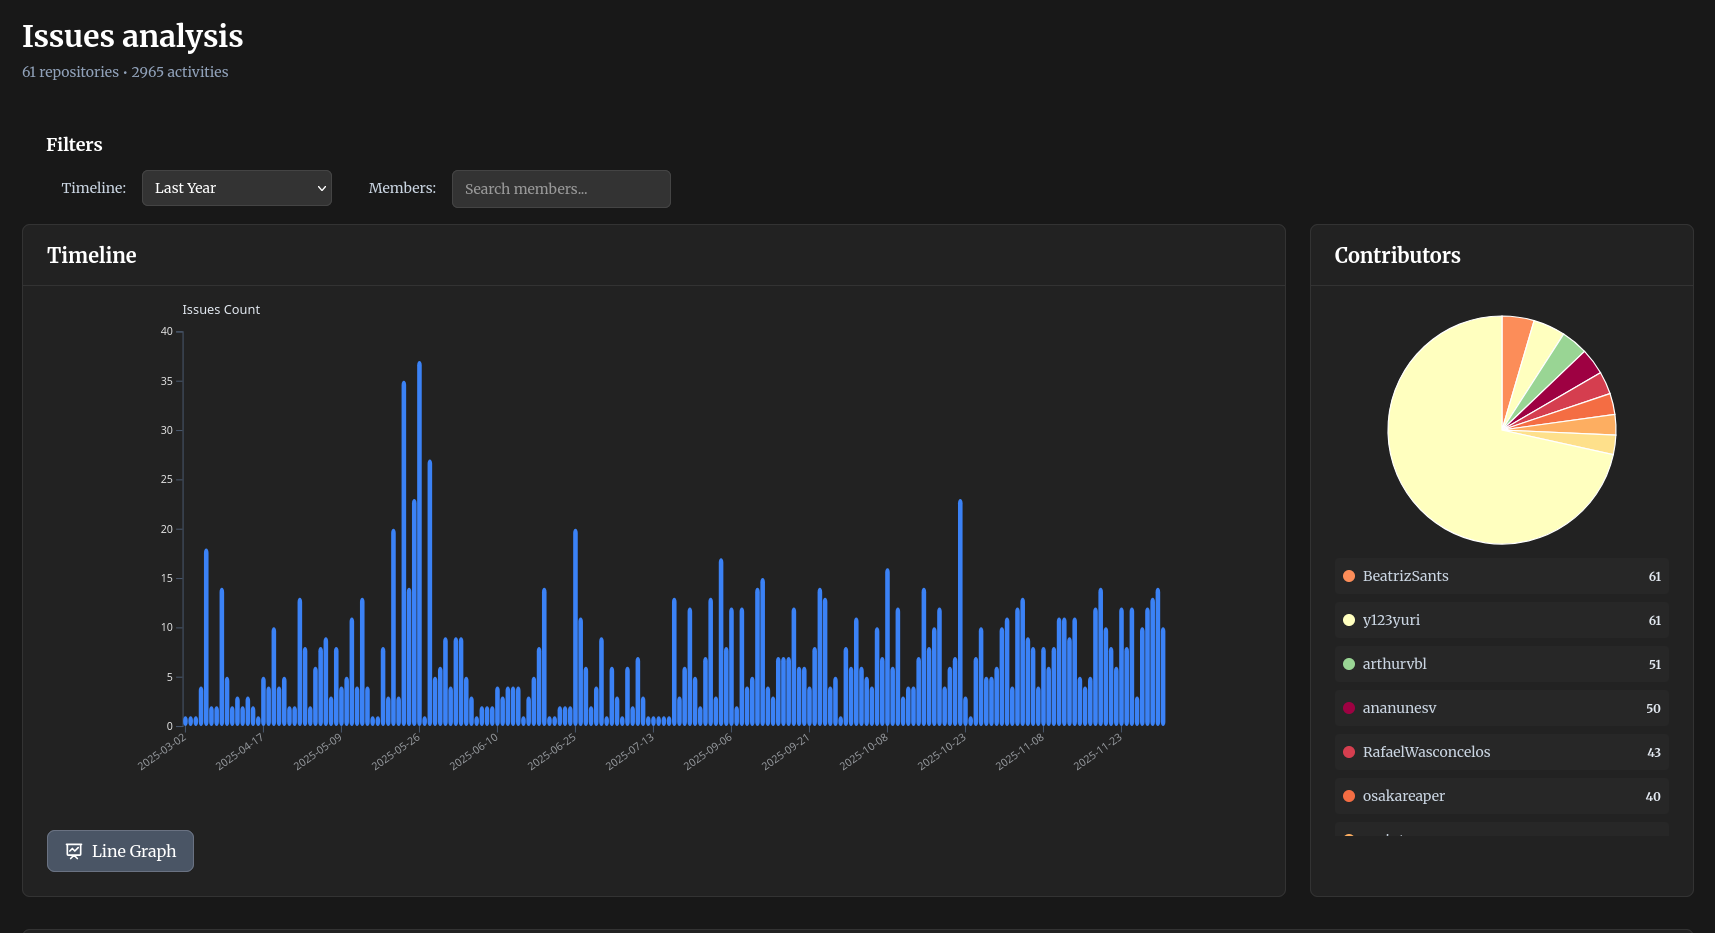
\includegraphics[width=0.9\textwidth]{screenshot-coops/issues-analysis-mds-with-contribution-pizza-graph.png}
\caption{Análise de issues de uma organização MDS com gráfico de distribuição de contribuições, demonstrando os KPIs de fluxo e participação.}
\label{fig:issues-kpis-coops}
\end{figure}

\begin{figure}[ht]
\centering
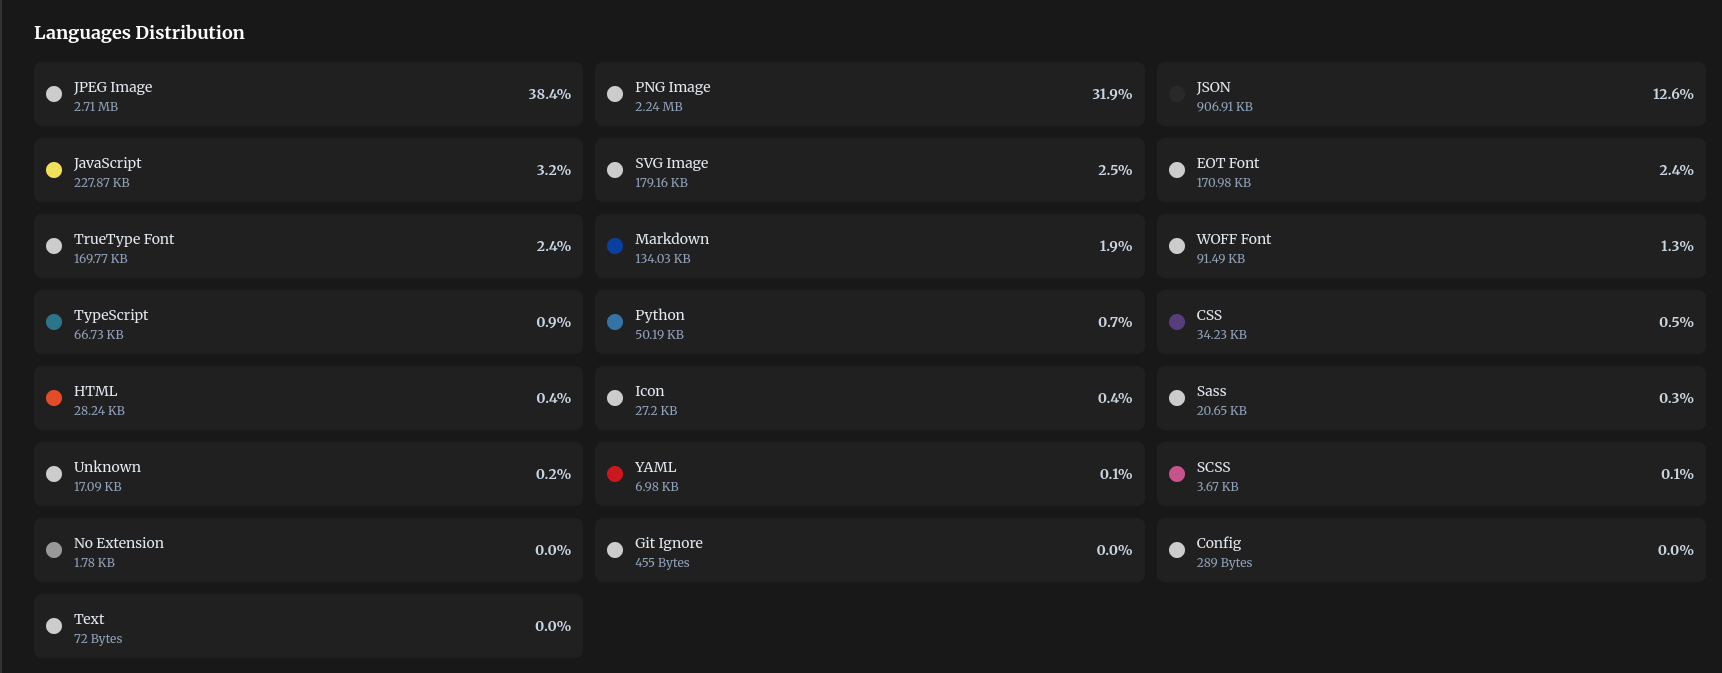
\includegraphics[width=0.9\textwidth]{screenshot-coops/language-distribution.png}
\caption{Distribuição de linguagens de programação nos repositórios da organização, com suporte a 90+ tipos de arquivo.}
\label{fig:language-distribution-coops}
\end{figure}

\subsection*{5.4 Análise por inteligência artificial}

O dashboard integra a API do \textbf{Google Gemini} para geração de resumos em linguagem natural:

\begin{itemize}
    \item Processamento em lote das contribuições de cada membro
    \item Geração de análises qualitativas automatizadas a partir dos dados Silver/Gold
    \item Degradação graciosa: quando a API não está disponível, a plataforma opera normalmente sem o módulo de IA
\end{itemize}

Este módulo foi adicionado durante as iterações com Dra.\ Carla Rocha, atendendo à necessidade de interpretações contextuais dos dados quantitativos.

\begin{figure}[ht]
\centering
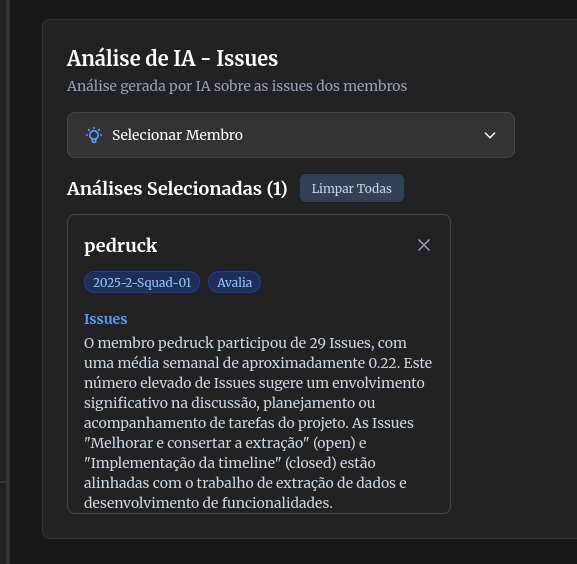
\includegraphics[width=0.9\textwidth]{screenshot-coops/ai-analysis-issues-from-one-member-from-mds.png}
\caption{Análise por IA (Google Gemini) das issues de um membro de equipe MDS, gerando resumo em linguagem natural das contribuições.}
\label{fig:ai-analysis-coops}
\end{figure}

\subsection*{5.5 Co-desenvolvimento e uso real}

O modelo de desenvolvimento do dashboard seguiu um processo de \textbf{co-desenvolvimento academia-academia}:

\begin{itemize}
    \item Danrley construiu a plataforma e colaborou diretamente com Dra.\ Carla Rocha (UnB) para definir quais dados das camadas Silver e Gold ela necessitava para suas disciplinas de MDS.
    \item O processo foi \textbf{iterativo}: Danrley e Carla decidiam juntos sobre métricas, visualizações e camadas de dados. A cada ciclo, novos módulos Silver/Gold eram implementados e validados.
    \item O módulo de \textbf{análise por IA} foi adicionado com base nas necessidades identificadas durante a colaboração.
    \item Ao final do semestre 2025/2, Dra.\ Carla \textbf{utilizou o dashboard para avaliar seus alunos} --- configurando uma validação pedagógica real do software.
    \item Duas instâncias em produção foram implantadas: UnB (\texttt{unb-mds.github.io}) e UDF (\texttt{labtechudf.github.io/CoOps}).
    \item A instância UnB analisa \textbf{70+ repositórios} da organização \texttt{unb-mds}, demonstrando a escalabilidade da solução.
\end{itemize}

\begin{figure}[ht]
\centering
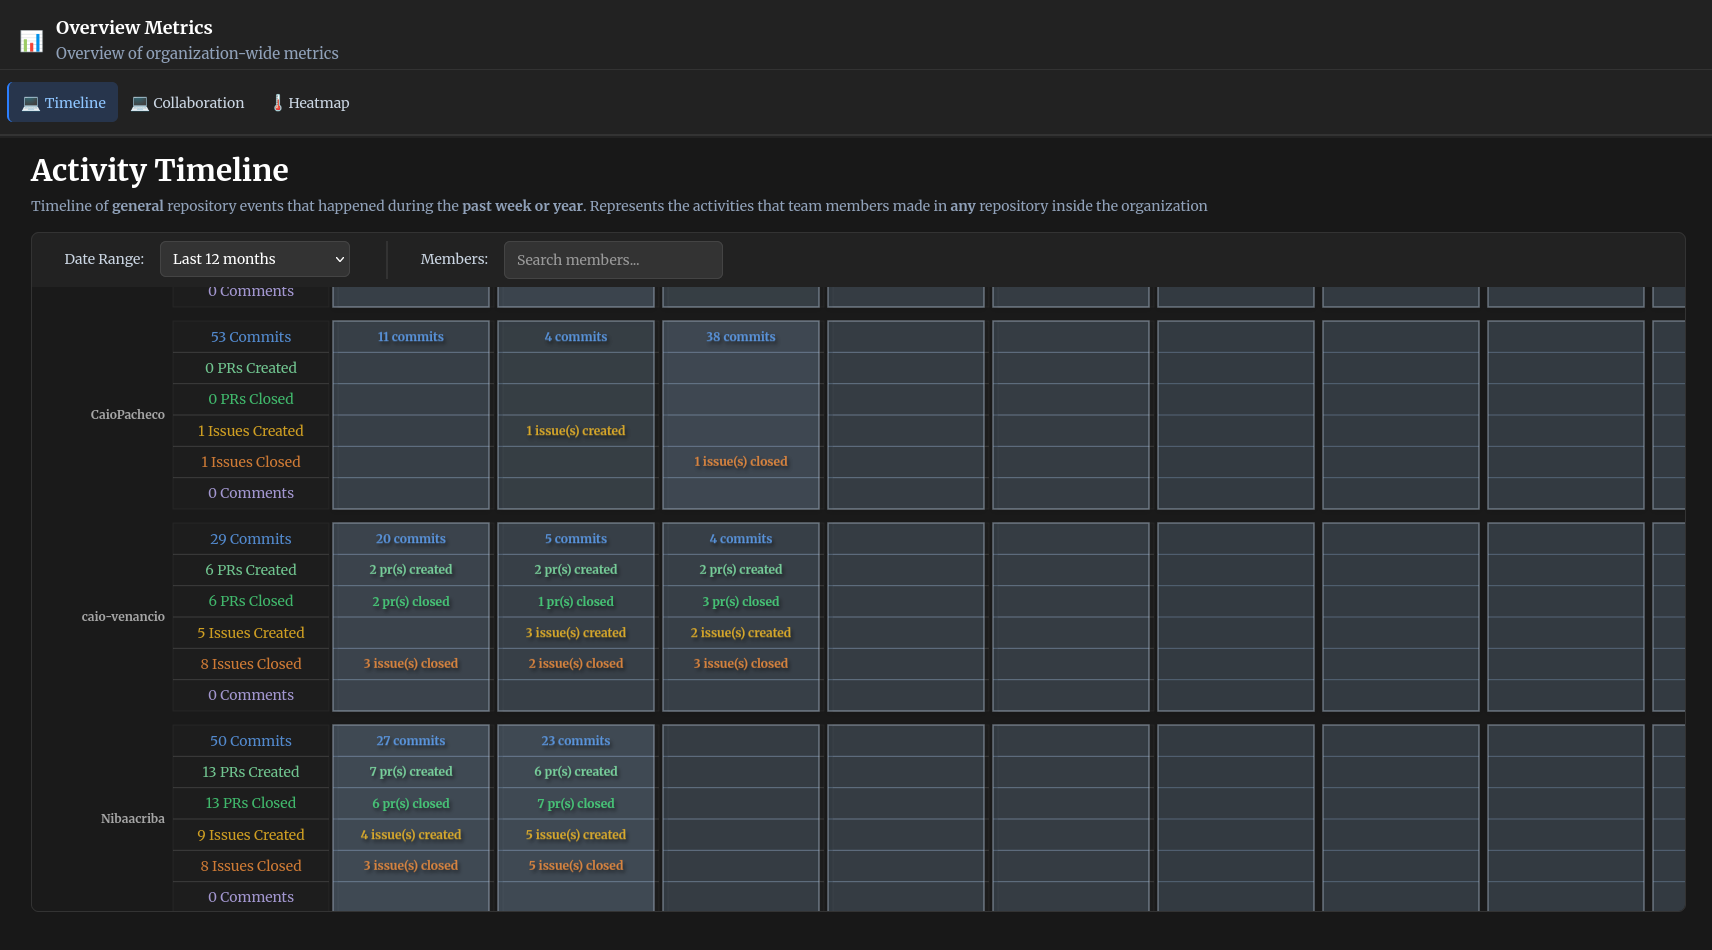
\includegraphics[width=0.9\textwidth]{screenshot-coops/activity-timeline-screen-partial-view-here-we-can-see-prs-issues-etc-by-user.png}
\caption{Timeline de atividade do dashboard analisando repositórios da organização unb-mds, com visualização de PRs, issues e contribuições por membro.}
\label{fig:timeline-unb-mds}
\end{figure}

\begin{figure}[ht]
\centering
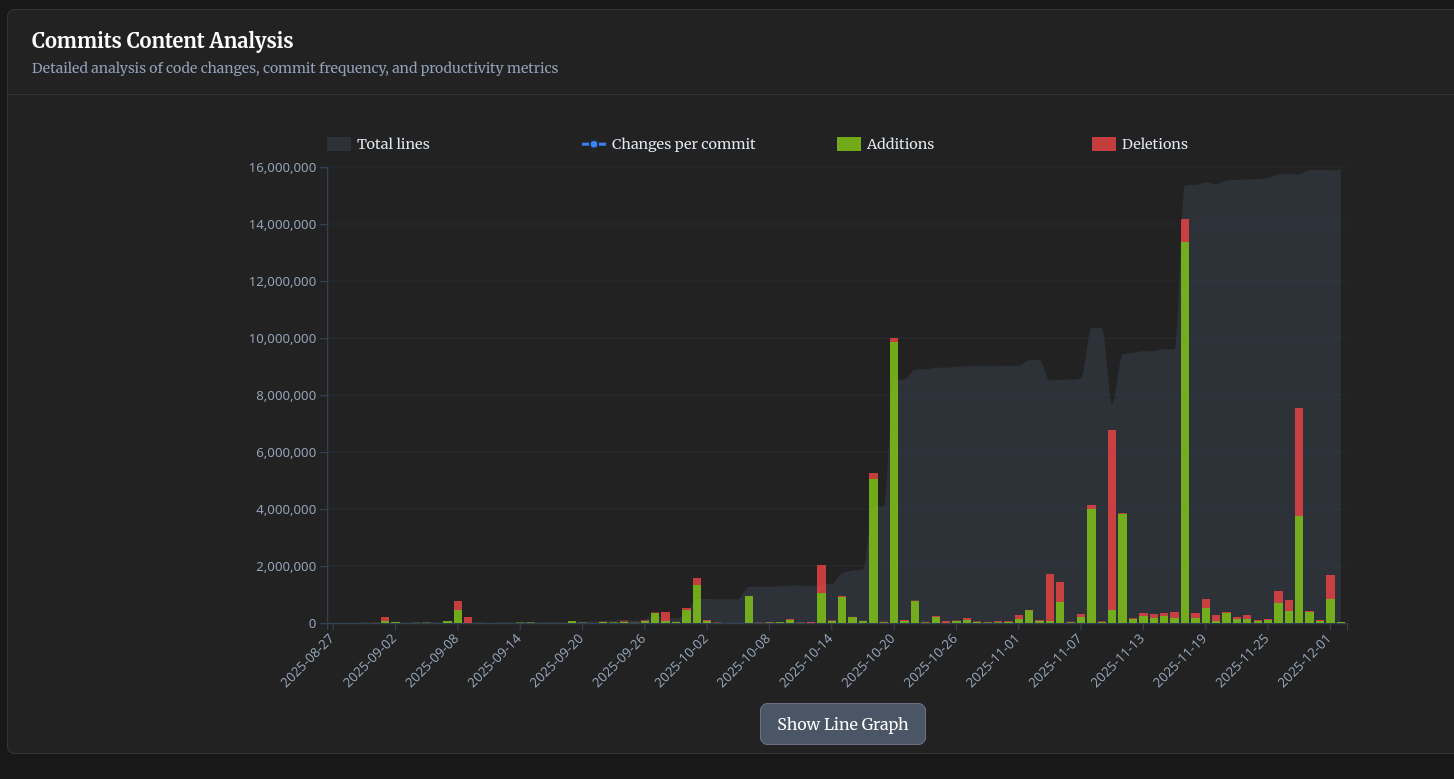
\includegraphics[width=0.9\textwidth]{screenshot-coops/commit-content-analysis-from-one-member-mds.png}
\caption{Análise de conteúdo de commits de um membro de equipe MDS, detalhando frequência, arquivos modificados e padrões de contribuição.}
\label{fig:commit-analysis-coops}
\end{figure}

\subsection*{5.6 KPIs implementados}

Os KPIs implementados no dashboard abrangem quatro dimensões:

\textbf{Técnicos:}
\begin{itemize}
    \item Commits por semana, code churn (linhas adicionadas/removidas)
    \item PR lead time (tempo de abertura ao merge), issue throughput (abertas/fechadas por período)
\end{itemize}

\textbf{Colaborativos:}
\begin{itemize}
    \item Participação em revisões de código, redes de colaboração (grafos)
    \item Concentração de contribuições (desigualdade), cross-collaboration entre repositórios
\end{itemize}

\textbf{Comportamentais:}
\begin{itemize}
    \item Activity heatmaps (padrões dia/hora), maturity scores
    \item Regularidade semanal (semanas ativas / total de semanas)
\end{itemize}

\textbf{Derivados de análise qualitativa:}
\begin{itemize}
    \item \textbf{Slope\_8w}: inclinação de contribuições nas primeiras 8 semanas (preditor de engajamento)
    \item \textbf{Clones\_W1--W2}: clones nas semanas iniciais como indicador de adesão
    \item \textbf{Centralidade}: posição nos grafos de interação (integrador vs.\ especialista)
    \item \textbf{Regularidade semanal}: constância de contribuições ao longo do semestre
\end{itemize}

\textbf{Classificação de desempenho}: os membros são categorizados em tiers --- top performers, regulares, ocasionais e não-contribuidores --- com base na combinação dos indicadores acima.

\subsection*{5.7 Testes e qualidade}

\begin{itemize}
    \item \textbf{Frontend}: \textbf{94\% de cobertura} de testes com Vitest + React Testing Library
    \item \textbf{Backend}: testes unitários e de integração com pytest
    \item \textbf{CI/CD}: GitHub Actions executa o pipeline diariamente às 5h UTC, incluindo extração de dados, transformação e deploy automático
    \item \textbf{Qualidade de código}: linting (ESLint, Ruff) integrado ao pipeline
\end{itemize}

\subsection*{5.8 Open source e replicabilidade}

\begin{itemize}
    \item \textbf{Licença}: GPL v3.0 --- garante que derivações permaneçam abertas
    \item \textbf{Suporte a linguagens}: 90+ tipos de arquivo/linguagem reconhecidos na análise de estrutura
    \item \textbf{Documentação}: CONTRIBUTING.md, ARQUITETURA.md e EXTRACAO\_DADOS.md disponíveis no repositório
    \item \textbf{Infraestrutura zero}: deploy via GitHub Pages, sem necessidade de servidores, bancos de dados ou custos de hospedagem
    \item \textbf{Replicação}: qualquer instituição pode fazer fork do repositório, configurar seus tokens e ter uma instância funcional em minutos
\end{itemize}

% ----------------------------------------------------------
% 6. ANÁLISES E DISCUSSÕES
% ----------------------------------------------------------
\section*{6.\ Análises e Discussões}

\textbf{Validação da Arquitetura Medalhão em contexto acadêmico.} A implementação completa das três camadas (Bronze$\rightarrow$Silver$\rightarrow$Gold) confirmou a adequação desse paradigma de engenharia de dados ao cenário de fábricas de software acadêmicas. A separação em camadas permite que usuários avançados (pesquisadores) acessem dados Bronze/Silver para análises customizadas, enquanto docentes e coordenadores consomem os KPIs Gold prontos via dashboard \cite{barbosaGeracaoGitHub,oliveira2022plataforma}.

\textbf{Co-desenvolvimento como modelo eficaz.} O modelo de co-desenvolvimento com Dra.\ Carla Rocha demonstrou-se eficaz: as iterações conjuntas sobre dados Silver/Gold garantiram que as métricas e visualizações atendessem a necessidades reais de avaliação pedagógica. Esse resultado é consonante com a literatura sobre co-criação academia-indústria \cite{bjerregaard2021lessons} e coordenação temporal em projetos colaborativos \cite{franssen2019cogs}.

\textbf{Validação pedagógica real.} O fato de Dra.\ Carla ter utilizado o dashboard para avaliar seus alunos ao final do semestre constitui a evidência mais forte da utilidade prática da plataforma. Essa validação vai além de testes-piloto controlados --- trata-se de uso real, em contexto pedagógico autêntico, com dezenas de equipes e 70+ repositórios.

\textbf{Maturidade técnica.} A otimização de \textbf{100x no desempenho} da extração (de 3--4 horas para 30--40 segundos) demonstra evolução técnica significativa. A migração de GraphQL para REST API, embora contraintuitiva, mostrou-se superior para o caso de uso específico de extração em lote de organizações GitHub.

\textbf{De protótipos estáticos a dashboard interativo.} O projeto evoluiu das 20 visualizações estáticas do Jupyter notebook (relatório parcial) para 13+ páginas interativas com D3.js, incluindo grafos de rede, treemaps, heatmaps e análise por IA. Essa evolução representa um salto qualitativo no potencial de análise disponível para docentes.

\textbf{Escalabilidade comprovada.} A instância UnB, analisando 70+ repositórios da organização \texttt{unb-mds}, demonstra que a solução escala para cenários reais de múltiplas equipes. O pipeline diário automatizado garante dados atualizados sem intervenção manual.

\textbf{Triangulação qualitativa.} Os dados qualitativos (Apêndices A e B) foram validados pelos dados quantitativos: a importância de métricas de ramp-up (Slope\_8w), clones iniciais, grafos de colaboração e regularidade semanal --- todos incorporados como KPIs no dashboard --- confirmou-se na prática com as turmas de Dra.\ Carla \cite{hamer2021using,kitchenham2010s}.

\textbf{Democratização via arquitetura serverless.} O dashboard demonstra que uma arquitetura serverless (GitHub Actions + GitHub Pages) pode democratizar o acesso a analytics avançados: custo zero, sem infraestrutura para manter, replicável por qualquer instituição. Isso remove barreiras técnicas e financeiras que historicamente limitaram a adoção de ferramentas de monitoramento em contextos acadêmicos \cite{vega2022scrumwatch,ozkan2019agile}.

\textbf{Relevância para a indústria.} Além do contexto acadêmico, o pipeline de dados reproduzível e de custo zero é aplicável a qualquer organização GitHub. Empresas podem utilizar o dashboard para monitorar equipes de desenvolvimento com as mesmas métricas e visualizações, sem investimento em infraestrutura.

\textbf{Relevância para a academia.} O dashboard possibilita avaliação pedagógica baseada em evidências --- permitindo que docentes identifiquem padrões de colaboração, acompanhem evolução temporal e fundamentem notas em dados objetivos, sem depender exclusivamente de percepções subjetivas \cite{oliveira2017conduccao,dos2021experiencia}.

% ----------------------------------------------------------
% 7. CONCLUSÃO
% ----------------------------------------------------------
\section*{7.\ Conclusão}

O projeto PIBIT superou o escopo originalmente proposto: de um protótipo de coleta e visualização, evoluiu para o \textbf{Dashboard de Monitoramento de Métricas de Produtividade e Qualidade} --- uma plataforma \textit{full-stack} em produção, validada e utilizada em contexto pedagógico real. O dashboard foi implantado e validado em \textbf{duas instituições} (UnB e UDF), demonstrando sua aplicabilidade e escalabilidade.

O modelo de co-desenvolvimento com Dra.\ Carla Rocha (UnB) mostrou-se eficaz: as iterações conjuntas sobre dados Silver e Gold, culminando na adição do módulo de análise por IA, produziram uma ferramenta que atende a necessidades reais de docentes que coordenam fábricas de software acadêmicas. A validação mais expressiva foi o \textbf{uso real para avaliação de alunos} ao final do semestre --- confirmando a relevância pedagógica do dashboard.

Do ponto de vista técnico, o dashboard demonstra que práticas de engenharia de dados da indústria (Arquitetura Medalhão, CI/CD, deploy serverless) podem ser aplicadas com sucesso ao contexto acadêmico. A otimização de 100x no pipeline, os 94\% de cobertura de testes e a arquitetura de infraestrutura zero evidenciam a maturidade técnica alcançada.

A distribuição sob licença \textbf{GPL v3.0} e a documentação abrangente (CONTRIBUTING.md, ARQUITETURA.md, EXTRACAO\_DADOS.md) garantem que outras instituições possam replicar e adaptar o dashboard às suas necessidades.

\textbf{Trabalhos futuros}: expansão para mais instituições; incorporação de métricas de qualidade de código (complexidade ciclomática, cobertura de testes dos projetos analisados); predições baseadas em aprendizado de máquina para identificação precoce de equipes em risco; e integração com outras plataformas além do GitHub (GitLab, Bitbucket).

% ----------------------------------------------------------
% REFERÊNCIAS BIBLIOGRÁFICAS
% ----------------------------------------------------------
\bibliography{relatorio-final}

% ----------------------------------------------------------
% APÊNDICES
% ----------------------------------------------------------
\begin{apendicesenv}
\partapendices

\chapter{Entrevista com LAPPIS/UnB (FGA)}
\label{apendiceA}

\textbf{Participantes:} Danrley Pereira (PIBIT/UDF) e Dra.\ Carla Rocha (Coordenadora LAPPIS) \\
\textbf{Data:} 22/08/2025 \\
\textbf{Local:} FGA -- UnB \\
\textbf{Tema:} Fábricas de software acadêmicas, métricas de interação e experiências do LAPPIS

\section*{1.\ Contexto Institucional}
\begin{itemize}
\item Envolvimento atual em \textbf{sistemas estruturantes} para controle orçamentário no poder executivo.
\item Desafio de \textbf{fragmentação de sistemas} e baixa interoperabilidade.
\end{itemize}

\section*{2.\ Reflexões sobre o modelo de ``Fábrica de Software''}
\begin{itemize}
\item Crítica ao conceito tradicional para ambientes acadêmicos/inovadores; necessidade de \textbf{repensar e adaptar} práticas ao aprendizado.
\end{itemize}

\section*{3.\ Arquitetura e tratamento de dados}
\begin{itemize}
\item Proposta da \textbf{Arquitetura Medalhão}:
\begin{itemize}
\item \textbf{Bronze (Raw):} extração de GitHub, GitLab, Notion;
\item \textbf{Silver:} transformação e homogeneização em modelos definidos;
\item \textbf{Gold:} camada de conhecimento com insights consolidados.
\end{itemize}
\item \textbf{Atualização semanal} considerada suficiente para o dashboard.
\end{itemize}

\section*{4.\ Métricas Quantitativas e Qualitativas}
\begin{itemize}
\item Necessidade de \textbf{interpretar quantitativos via análises qualitativas}.
\end{itemize}

\section*{5.\ Formação Acadêmica e Experiência}
\begin{itemize}
\item Disciplinas regulares: \textbf{4 meses}; alunos ingressam a partir do \textbf{4º semestre} e permanecem, em média, \textbf{2 anos}.
\end{itemize}

\section*{6.\ Métricas de Interações em Repositórios}
\begin{itemize}
\item Potencial de \textbf{grafos de rede} para mapear perfis:
\begin{itemize}
\item \textit{Aluno integrador}: muitos vínculos entre membros/repos;
\item \textit{Aluno especialista}: foco em áreas específicas (ex.: SRE/DevOps).
\end{itemize}
\end{itemize}

\section*{7.\ Conclusões e Próximos Passos}
\begin{itemize}
\item Alinhamento sobre utilidade de \textbf{métricas de interação} e adoção do modelo em \textbf{camadas (Bronze~$\rightarrow$~Silver~$\rightarrow$~Gold)}.
\item Reforço da \textbf{integração de contexto qualitativo} às análises.
\end{itemize}

\chapter{Relatos LABTECH/UDF}
\label{apendiceB}

\section*{Resumo dos relatos}
\begin{itemize}
\item No início do semestre, \textbf{interações no GitHub tendem a ser tímidas}, pois os alunos ainda estão se ambientando ao projeto e ao domínio.
\item A \textbf{curva inicial} pode ser mais baixa, com \textbf{aceleração ao redor da metade do semestre}.
\item \textbf{Commits e interações} mostram quem efetivamente contribuiu e buscou engajar.
\item O \textbf{número de \textit{clones}} no começo do semestre sinaliza a \textbf{intenção de participação}; acompanhar sua evolução pode indicar adesão.
\end{itemize}

\section*{Implicações para os KPIs}
\begin{itemize}
\item Monitorar a \textbf{inclinação inicial} (semanas 1--8) como possível preditor de sucesso posterior.
\item Persistir e analisar \textbf{clones} no início (\emph{traffic/clones}) como indicador de intenção.
\item Separar leituras por \textbf{papéis} (autor, revisor) e por \textbf{áreas} (dados, frontend, APIs, plataforma), permitindo distinguir \textit{integradores} de \textit{especialistas}.
\end{itemize}


\chapter{Análise de Dados GitHub do LabTech}
\label{apendiceC}

\section*{Contexto}
Este apêndice resume a exploração de scripts e sua execução para coleta e análise de dados da organização \texttt{LabTechUDF} no GitHub, servindo como base para construção do dashboard.

\section*{Como os dados foram capturados}
A pipeline implementa um \textbf{ETL} completo com:
\begin{itemize}
    \item Coleta via \textbf{GitHub API} da organização \texttt{LabTechUDF};
    \item \textbf{Cache} para evitar chamadas desnecessárias e \textbf{rate limit monitoring};
    \item \textbf{Filtragem} automática (remoção de \textit{forks} e \textit{blacklist} de repositórios);
    \item Coletas abrangentes: dados organizacionais e membros; repositórios e colaboradores; \textit{issues}, \textit{pull requests} e eventos; \textit{commits} e \textit{timeline}; \textbf{mapeamento de relacionamentos} entre contribuidores.
\end{itemize}

\section*{Arquitetura de dados (Medalhão)}
\begin{itemize}
    \item \textbf{Bronze (raw)}: ingestão \emph{append-only} dos JSONs de origem (GitHub), preservando \textit{payloads}, carimbos de tempo e metadados;
    \item \textbf{Silver (cleaned/modelado)}: normalização em modelos tabulares (\texttt{dim\_repos}, \texttt{dim\_users}, \texttt{fact\_commits}, \texttt{fact\_prs}, \texttt{fact\_issues}, \texttt{fact\_reviews}), com padronização temporal e colunas de linhagem;
    \item \textbf{Gold (métricas/KPIs)}: agregações para o \textit{dashboard} (throughput de \textit{issues}, \textit{lead time} de PR, \textit{code churn} semanal, participação em \textit{reviews}).
\end{itemize}

\section*{Métricas extraídas}
\textbf{Técnicas:} commits por usuário/repositório/tempo; \textit{issues} criadas/atribuídas/fechadas; \textit{PRs} abertos/revisados; \textit{cycle time} para \textit{issues}/\textit{PRs}; \textit{burndown}; \textit{code churn} e frequência de commits.

\noindent\textbf{Colaborativas:} rede de colaboração; \textit{cross-collaboration} (múltiplos repositórios); participação em \textit{reviews}/comentários; centralidade e papéis (integrador vs.\ especialista).

\noindent\textbf{Comportamentais:} \textit{activity heatmaps} (dia x hora); \textit{maturity score} (idade de conta, repositórios públicos, seguidores); perfil de membro (novo vs.\ estabelecido).

\section*{Visualizações geradas (protótipos iniciais --- 20)}
\begin{enumerate}
    \item \textit{activity-heatmap.png} --- Heatmap de atividade por dia/hora
    \item \textit{burndown-chart.png} --- Burndown de \textit{issues}
    \item \textit{collaboration-network.png} --- Rede de colaboração completa
    \item \textit{collaboration-network-no-isolated.png} --- Rede sem nós isolados
    \item \textit{commit-boxplot.png} --- Boxplot de distribuição de commits
    \item \textit{commit-frequency.png} --- Frequência de commits
    \item \textit{contributions-over-time.png} --- Contribuições ao longo do tempo
    \item \textit{contributions-over-time-filtered.png} --- Contribuições (Aug--Dec 2024)
    \item \textit{contributions-per-member.png} --- Contribuições por membro
    \item \textit{contributions-per-repo.png} --- Contribuições por repositório
    \item \textit{cross-collab-histogram.png} --- Colaboração cruzada
    \item \textit{cycle-time-histogram.png} --- Tempo de resolução de \textit{issues}
    \item \textit{established-contributions.png} --- Membros estabelecidos vs.\ contribuições
    \item \textit{github-usage-heatmap.png} --- Heatmap de uso do GitHub
    \item \textit{issue-states.png} --- Estados de \textit{issues} (abertas vs.\ fechadas)
    \item \textit{maturity-vs-contributions.png} --- Maturidade vs.\ contribuições
    \item \textit{new-pie-contribution.png} --- Novos membros vs.\ contribuições
    \item \textit{pie-contributions.png} --- Distribuição geral de contribuições
    \item \textit{pr-cycle-time-histogram.png} --- Tempo de resolução de PRs
    \item \textit{repos-followers.png} --- Repositórios públicos vs.\ seguidores
\end{enumerate}

\section*{Principais insights}
\begin{itemize}
    \item \textbf{Arquitetura medalhão} efetivamente implementada (Bronze~$\rightarrow$~Silver~$\rightarrow$~Gold);
    \item \textbf{Triangulação qualitativa} com os \textbf{Apêndices A e B} para interpretar variações das séries;
    \item KPIs específicos como \textbf{Slope\_8w} (ritmo inicial) e \textbf{centralidade} em grafos de interação;
    \item \textbf{Atualização semanal} suficiente para governança pedagógica;
    \item Identificação de \textbf{hubs} (membros que contribuem em múltiplos repositórios) e padrões de \textit{cross-collaboration}.
\end{itemize}

\section*{Reprodutibilidade e ética}
\begin{itemize}
    \item Código fonte disponível nos repositórios \texttt{LabTechUDF/CoOps} e \texttt{unb-mds/2025-2-Squad-01};
    \item Linhagem preservada (colunas de auditoria no Silver); KPIs recomputáveis;
    \item Anonimização de identificadores para divulgação acadêmica, conforme diretrizes éticas do projeto.
\end{itemize}

\section*{Visualizações representativas dos protótipos}

As figuras a seguir ilustram exemplos das 20 visualizações geradas na fase de prototipagem.

\begin{figure}[ht]
\centering
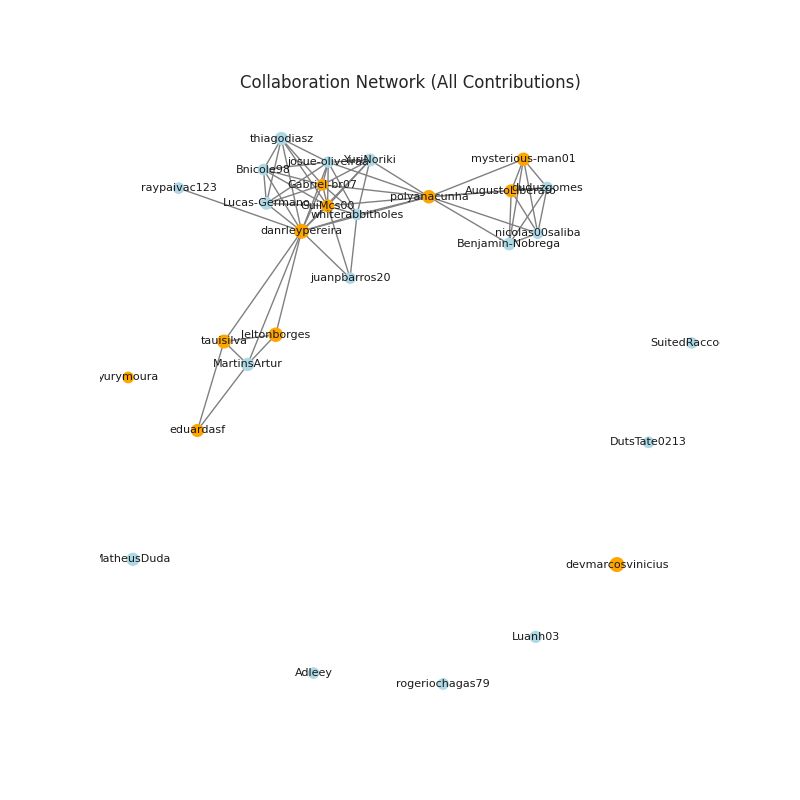
\includegraphics[width=0.8\textwidth]{collaboration-network.png}
\caption{Rede de colaboração da organização LabTechUDF. O grafo mostra as interações entre membros através de commits, issues e pull requests.}
\label{fig:collaboration-network}
\end{figure}

\begin{figure}[ht]
\centering
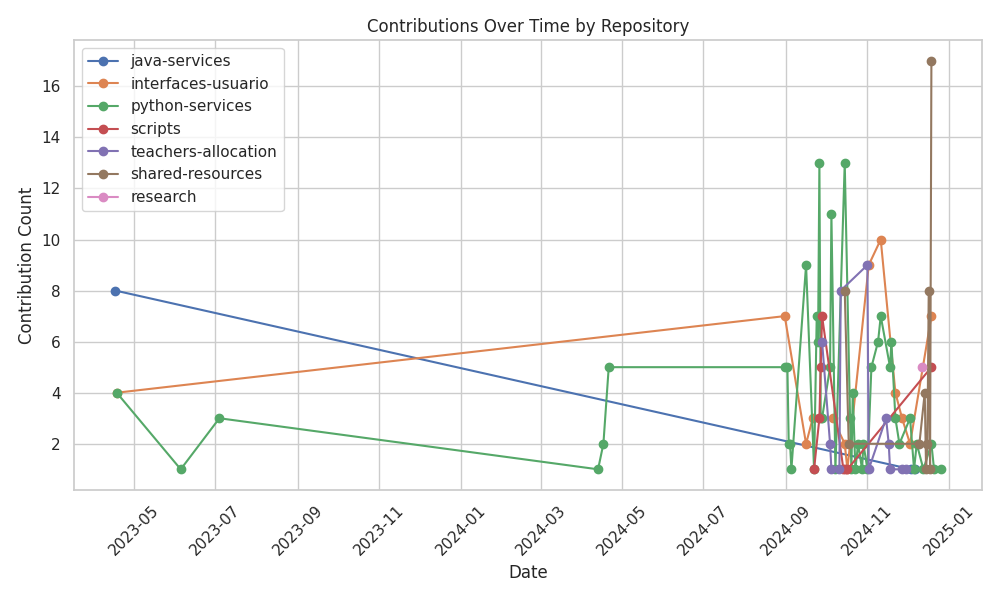
\includegraphics[width=0.8\textwidth]{contributions-over-time.png}
\caption{Evolução das contribuições ao longo do tempo por membro. A série temporal evidencia padrões de engajamento.}
\label{fig:contributions-over-time}
\end{figure}

\begin{figure}[ht]
\centering
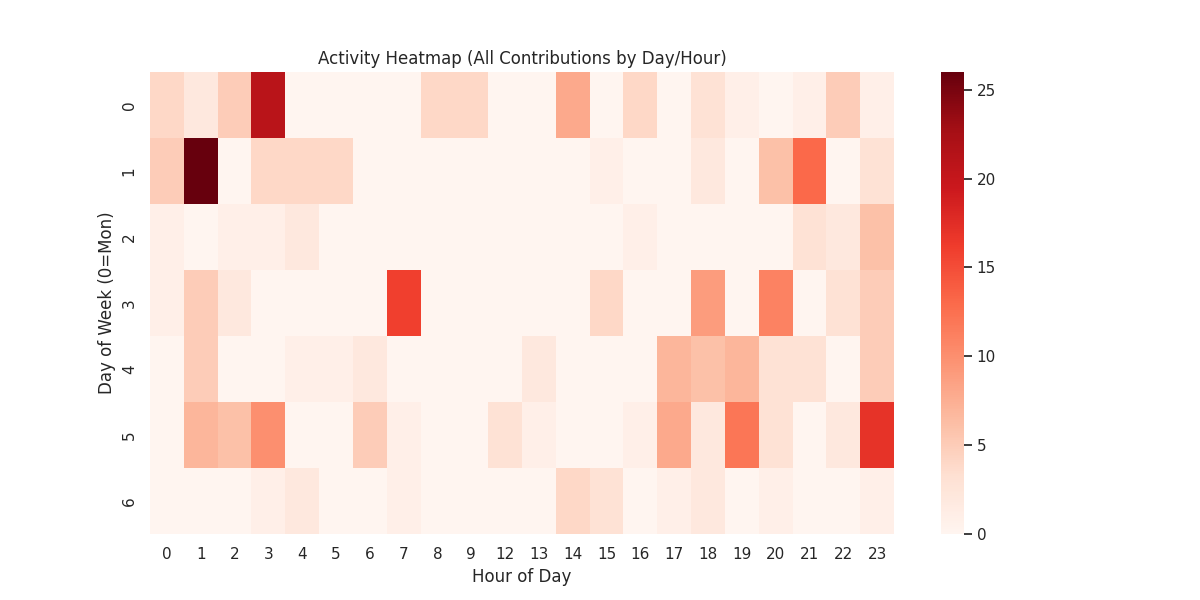
\includegraphics[width=0.8\textwidth]{activity-heatmap.png}
\caption{Heatmap de atividade por dia da semana e hora do dia.}
\label{fig:activity-heatmap}
\end{figure}

\begin{figure}[ht]
\centering
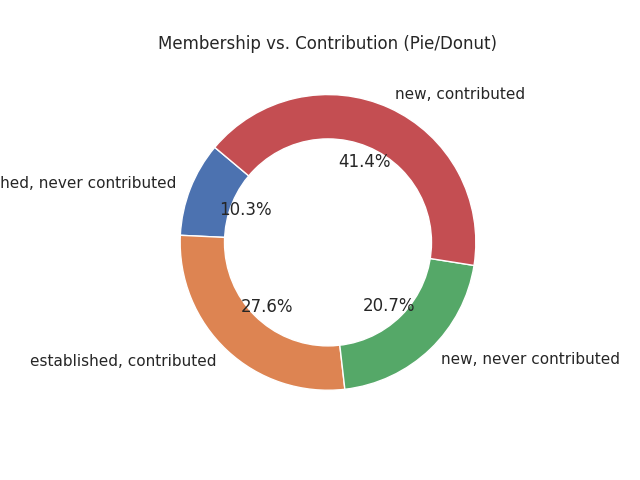
\includegraphics[width=0.8\textwidth]{pie-contributions.png}
\caption{Distribuição de contribuições por classes de membros da organização.}
\label{fig:pie-contributions}
\end{figure}


\chapter{Arquitetura e Funcionalidades do dashboard}
\label{apendiceD}

\section*{Topologia da aplicação}

O dashboard segue uma arquitetura serverless composta por:
\begin{itemize}
    \item \textbf{Pipeline Python} executado via GitHub Actions (extração, transformação, análise por IA)
    \item \textbf{Frontend React/TypeScript} servido via GitHub Pages
    \item \textbf{Dados JSON} versionados no repositório (Bronze/Silver/Gold)
    \item \textbf{Sem backend ativo}: toda a lógica de transformação é executada no pipeline CI/CD
\end{itemize}

A Figura~\ref{fig:arquitetura-geral} ilustra a topologia geral e a Figura~\ref{fig:dag-medalhao} detalha o DAG do pipeline Medalhão.

\begin{figure}[ht]
\centering

\includegraphics[width=0.9\textwidth]{arquitetura-geral.png}
\caption{Arquitetura geral da solução serverless. O diagrama mostra a integração entre stakeholders acadêmicos, processamento automatizado via GitHub Actions, armazenamento em camadas (Bronze/Silver/Gold) e frontend React servido via GitHub Pages.}
\label{fig:arquitetura-geral}
\end{figure}

\begin{figure}[ht]
\centering
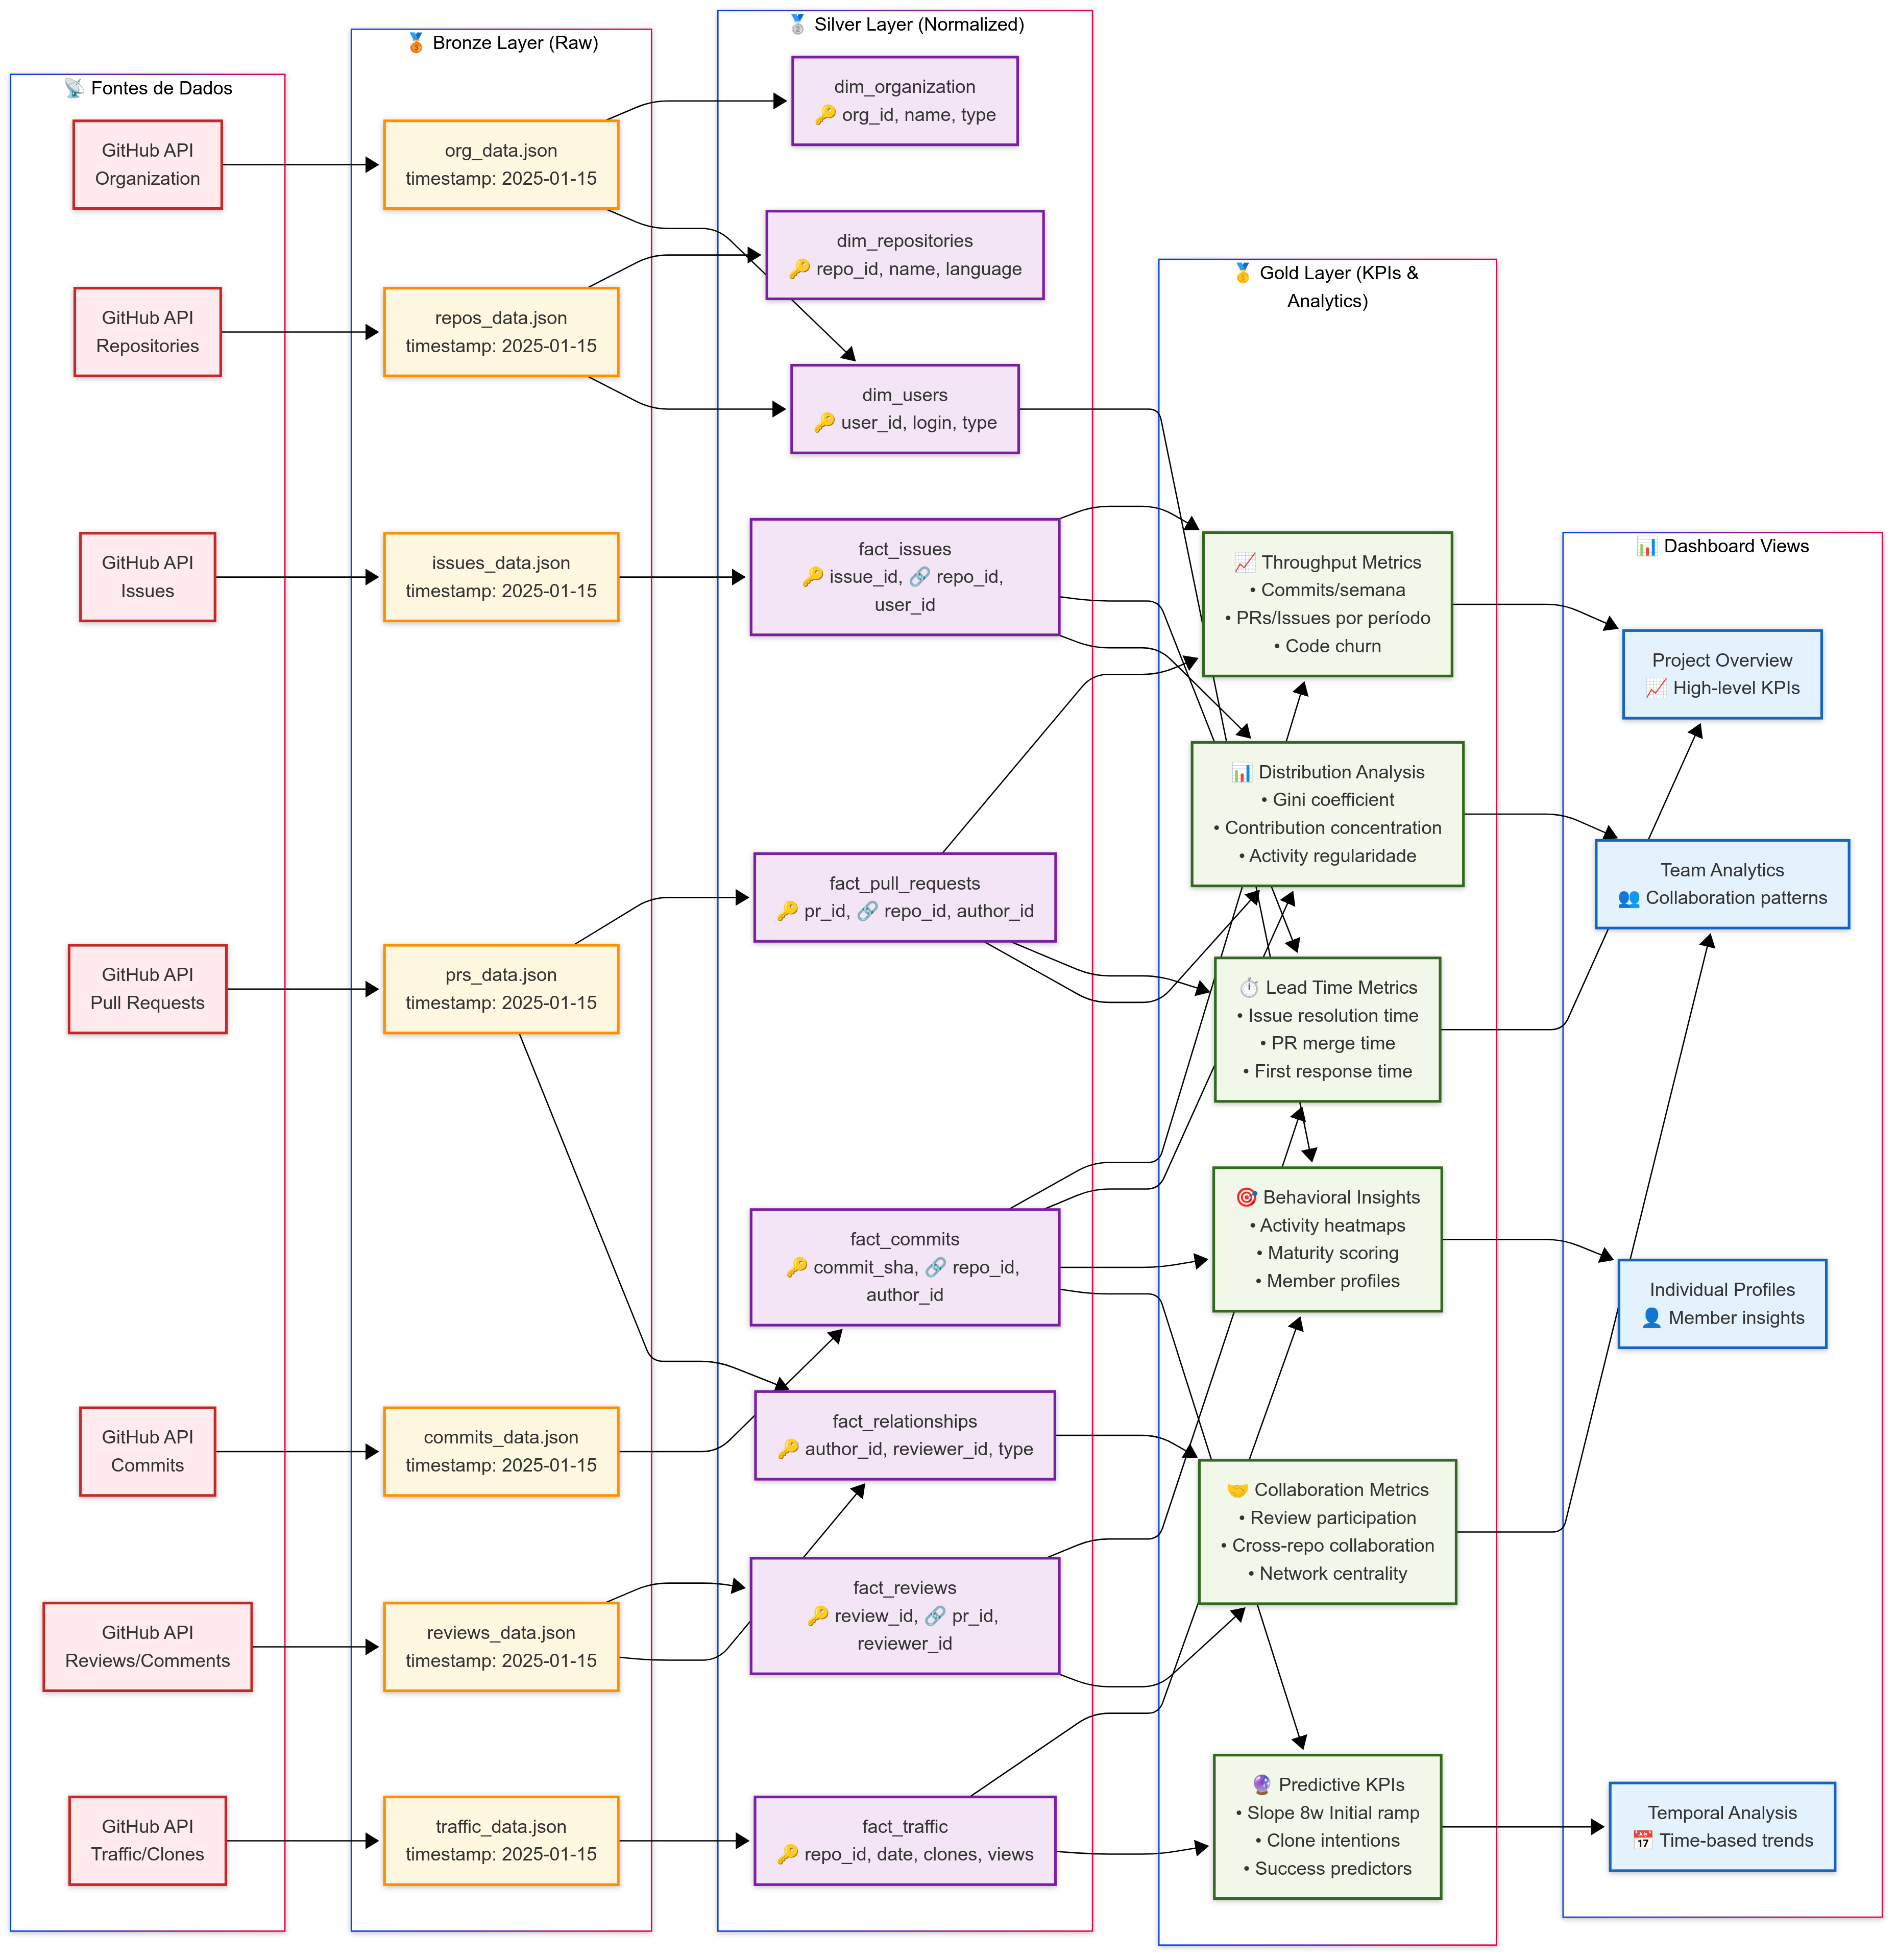
\includegraphics[width=0.9\textwidth]{dag-medalhao.png}
\caption{DAG da Arquitetura Medalhão detalhando o fluxo completo Bronze$\rightarrow$Silver$\rightarrow$Gold. As fontes GitHub API alimentam dados raw (Bronze), que são normalizados em tabelas dimensionais/fatos (Silver) e agregados em KPIs prontos para dashboard (Gold).}
\label{fig:dag-medalhao}
\end{figure}

\section*{Fluxo ETL}

O pipeline é executado diariamente às 5h UTC via GitHub Actions:
\begin{enumerate}
    \item \textbf{Extração Bronze}: chamadas à API REST do GitHub para 7 categorias de dados
    \item \textbf{Transformação Silver}: processamento em 6 módulos analíticos
    \item \textbf{Agregação Gold}: produção de KPIs executivos e classificação de desempenho
    \item \textbf{Análise por IA} (opcional): geração de resumos via API Google Gemini
    \item \textbf{Deploy}: commit dos dados processados e deploy automático via GitHub Pages
\end{enumerate}

A Figura~\ref{fig:sequencia-etl} ilustra o diagrama de sequência deste processo.

\begin{figure}[ht]
\centering
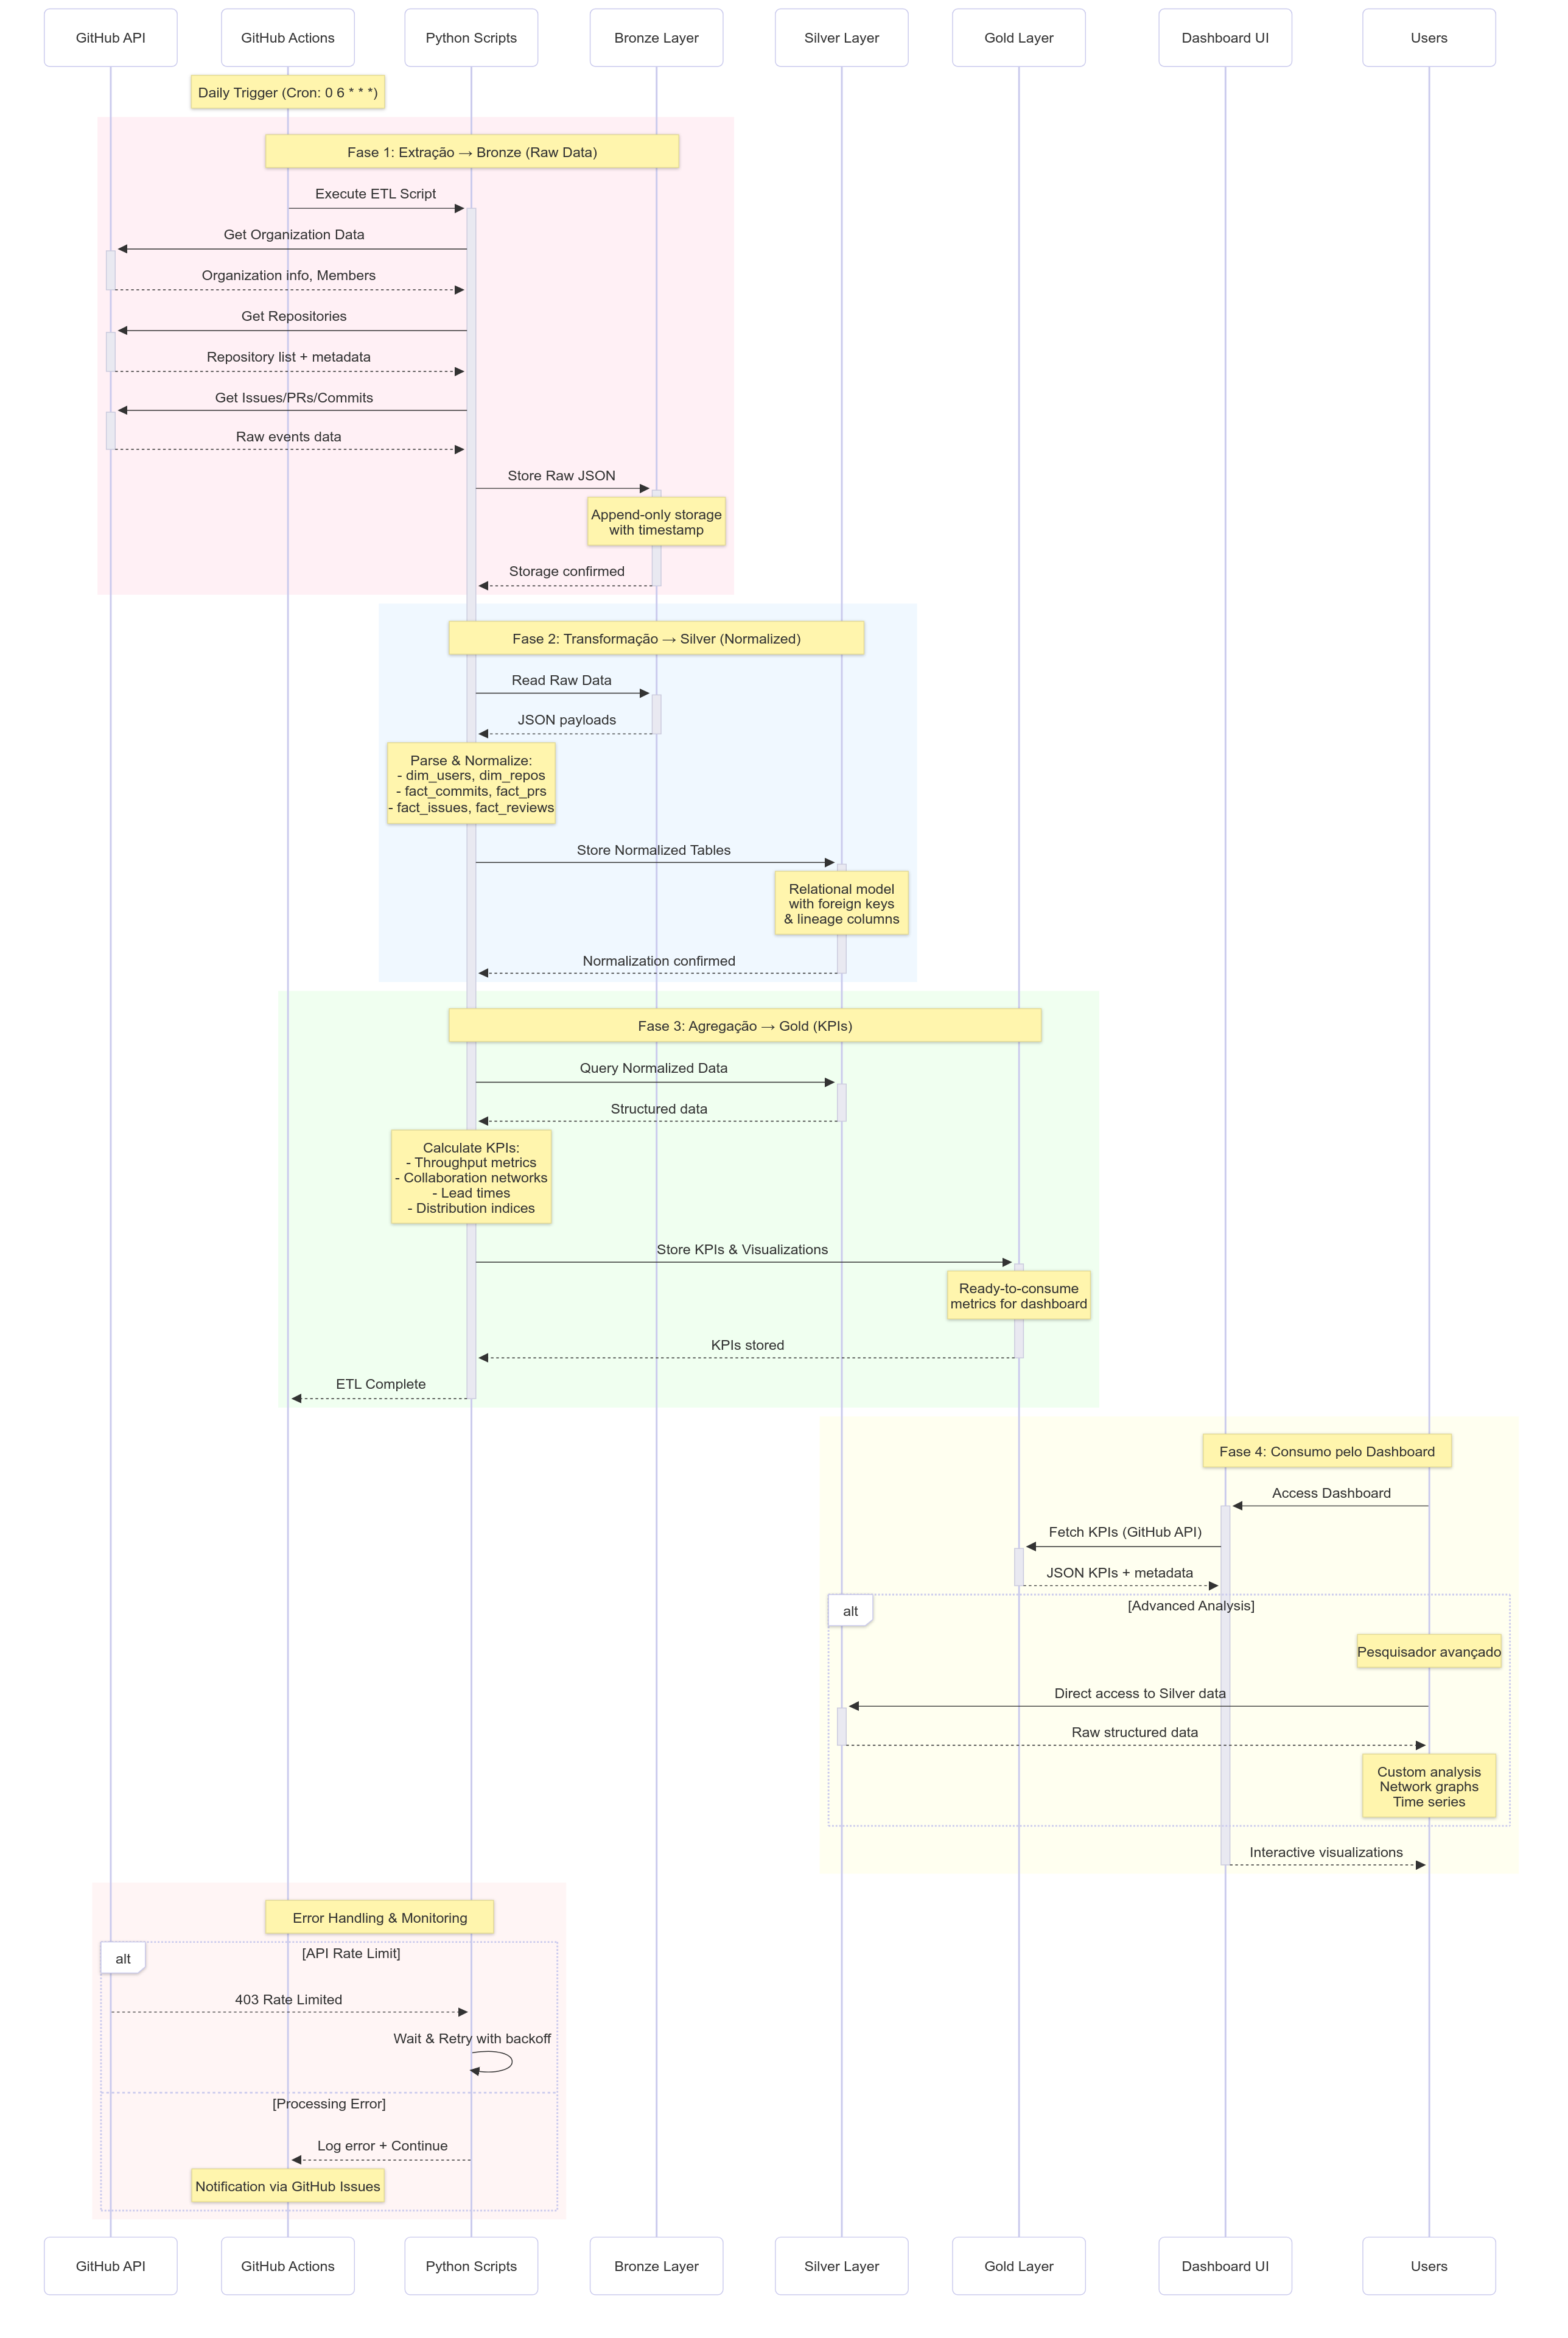
\includegraphics[width=0.9\textwidth]{sequencia_etl.png}
\caption{Diagrama de sequência do processo ETL automatizado. Ilustra as fases principais: extração via GitHub API, transformação Bronze$\rightarrow$Silver, agregação Silver$\rightarrow$Gold e consumo pelo dashboard.}
\label{fig:sequencia-etl}
\end{figure}

\section*{Principais funcionalidades do frontend}
\begin{itemize}
    \item Visualizações interativas D3.js com zoom, filtros e tooltips
    \item Páginas por repositório e por organização
    \item Análise individual de membros com resumo por IA
    \item Navegação entre camadas de dados (Silver $\rightarrow$ Gold)
    \item Design responsivo com Tailwind CSS
    \item Suporte a temas claro/escuro
\end{itemize}


\chapter{Galeria de Screenshots do dashboard}
\label{apendiceE}

As figuras a seguir apresentam capturas de tela adicionais da plataforma em operação, complementando as figuras inseridas ao longo do texto principal.

\begin{figure}[ht]
\centering
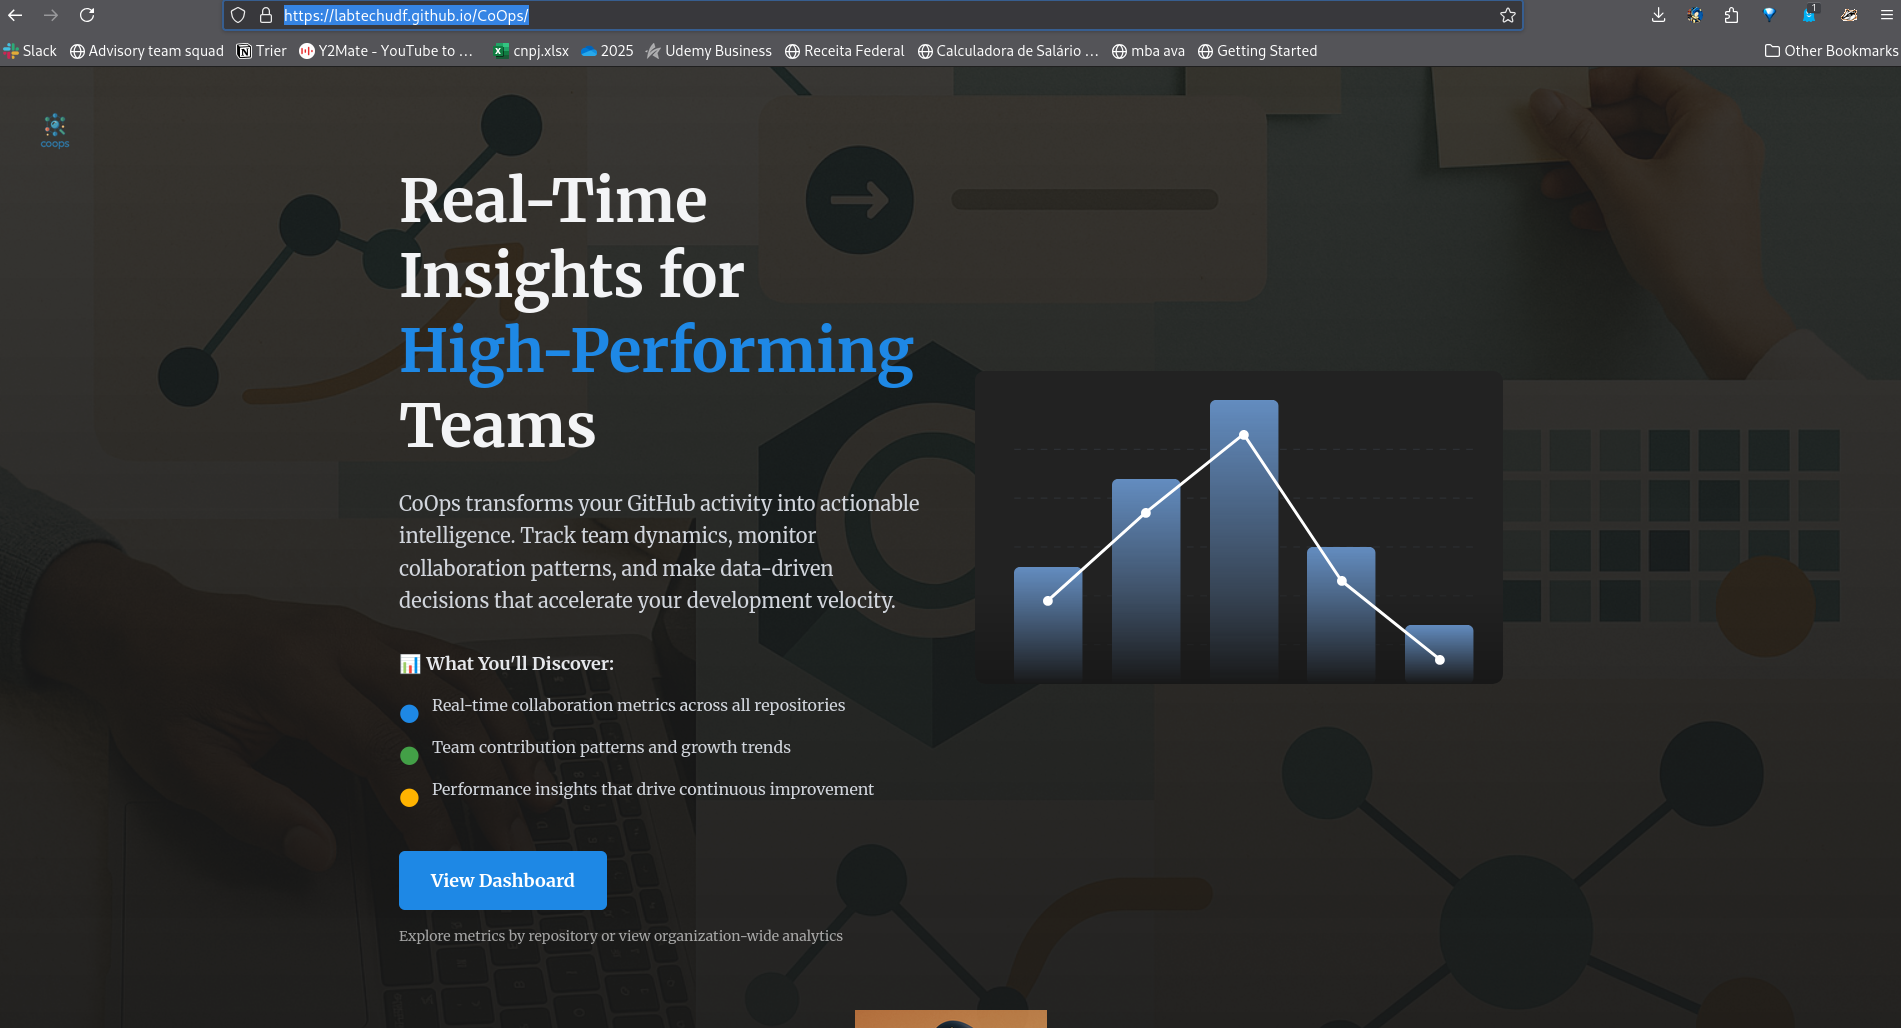
\includegraphics[width=0.9\textwidth]{screenshot-coops/pagina-inicial.png}
\caption{Página inicial do dashboard.}
\end{figure}

\begin{figure}[ht]
\centering
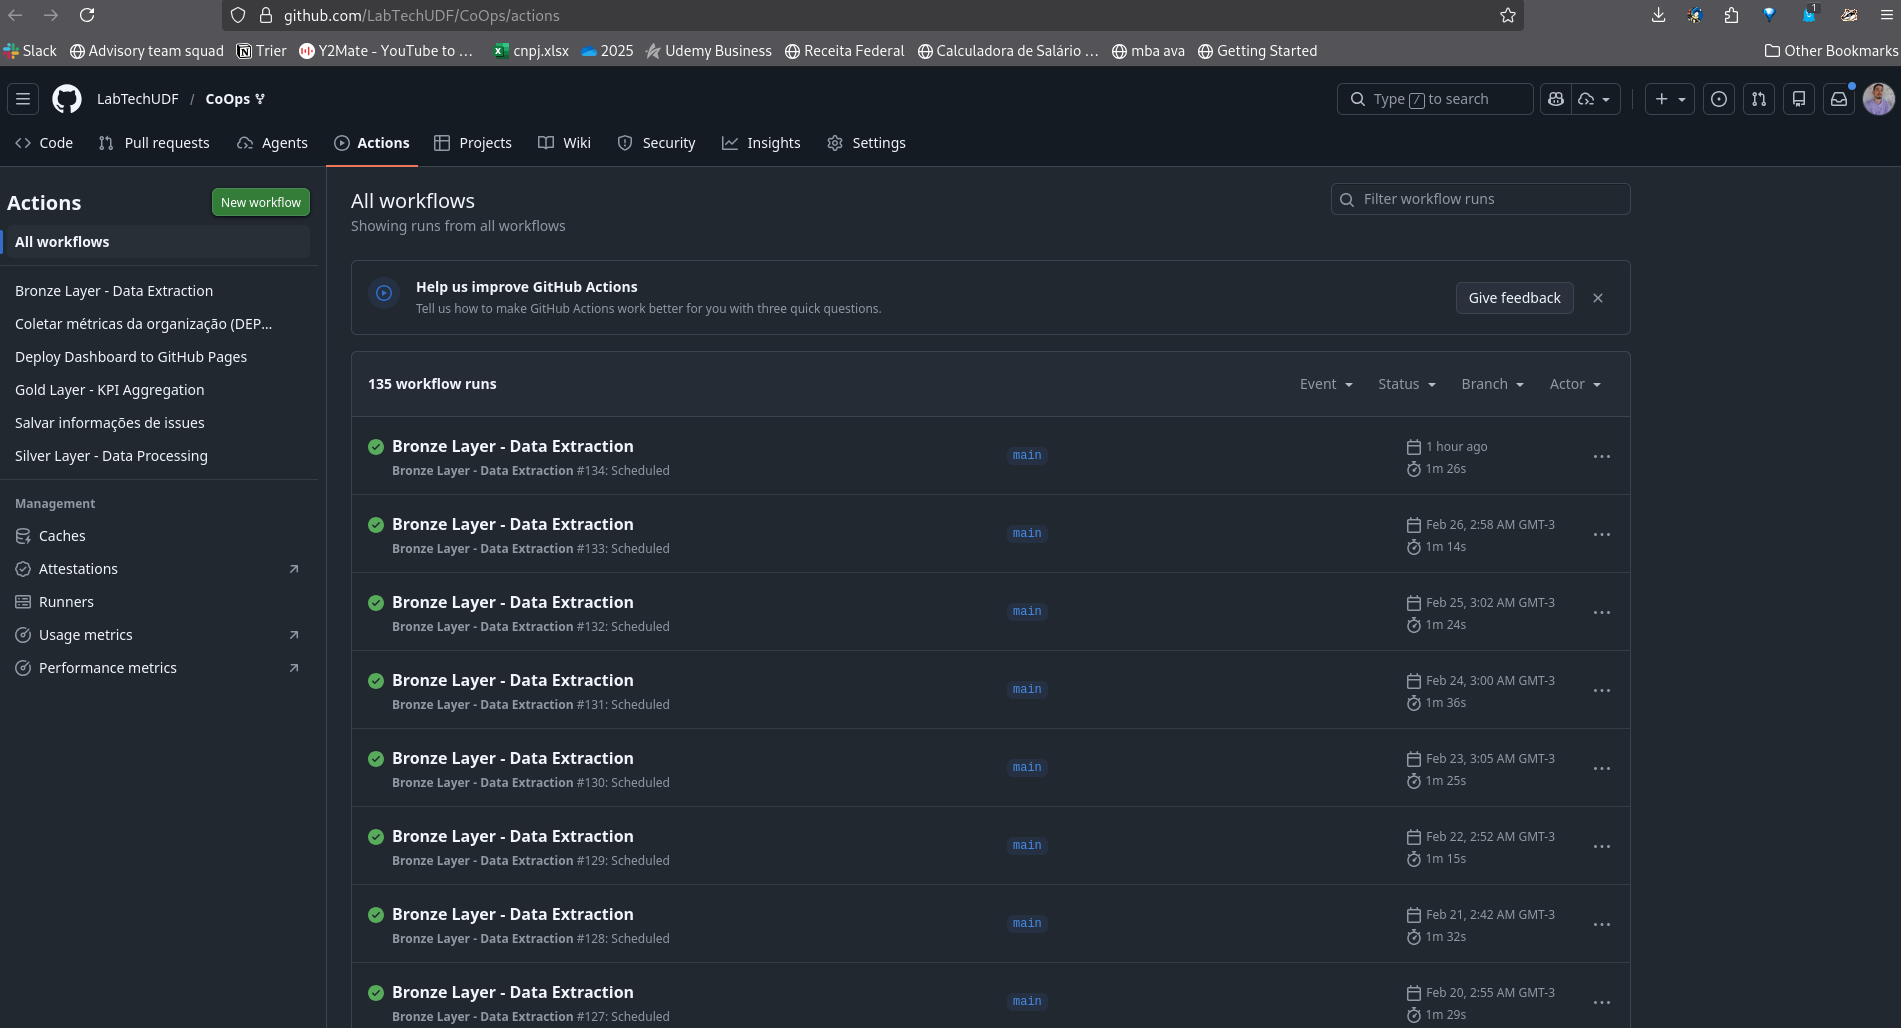
\includegraphics[width=0.9\textwidth]{screenshot-coops/pipelines-github-todos-workflows-rodados.png}
\caption{Histórico de execuções dos workflows no GitHub Actions.}
\end{figure}

\begin{figure}[ht]
\centering
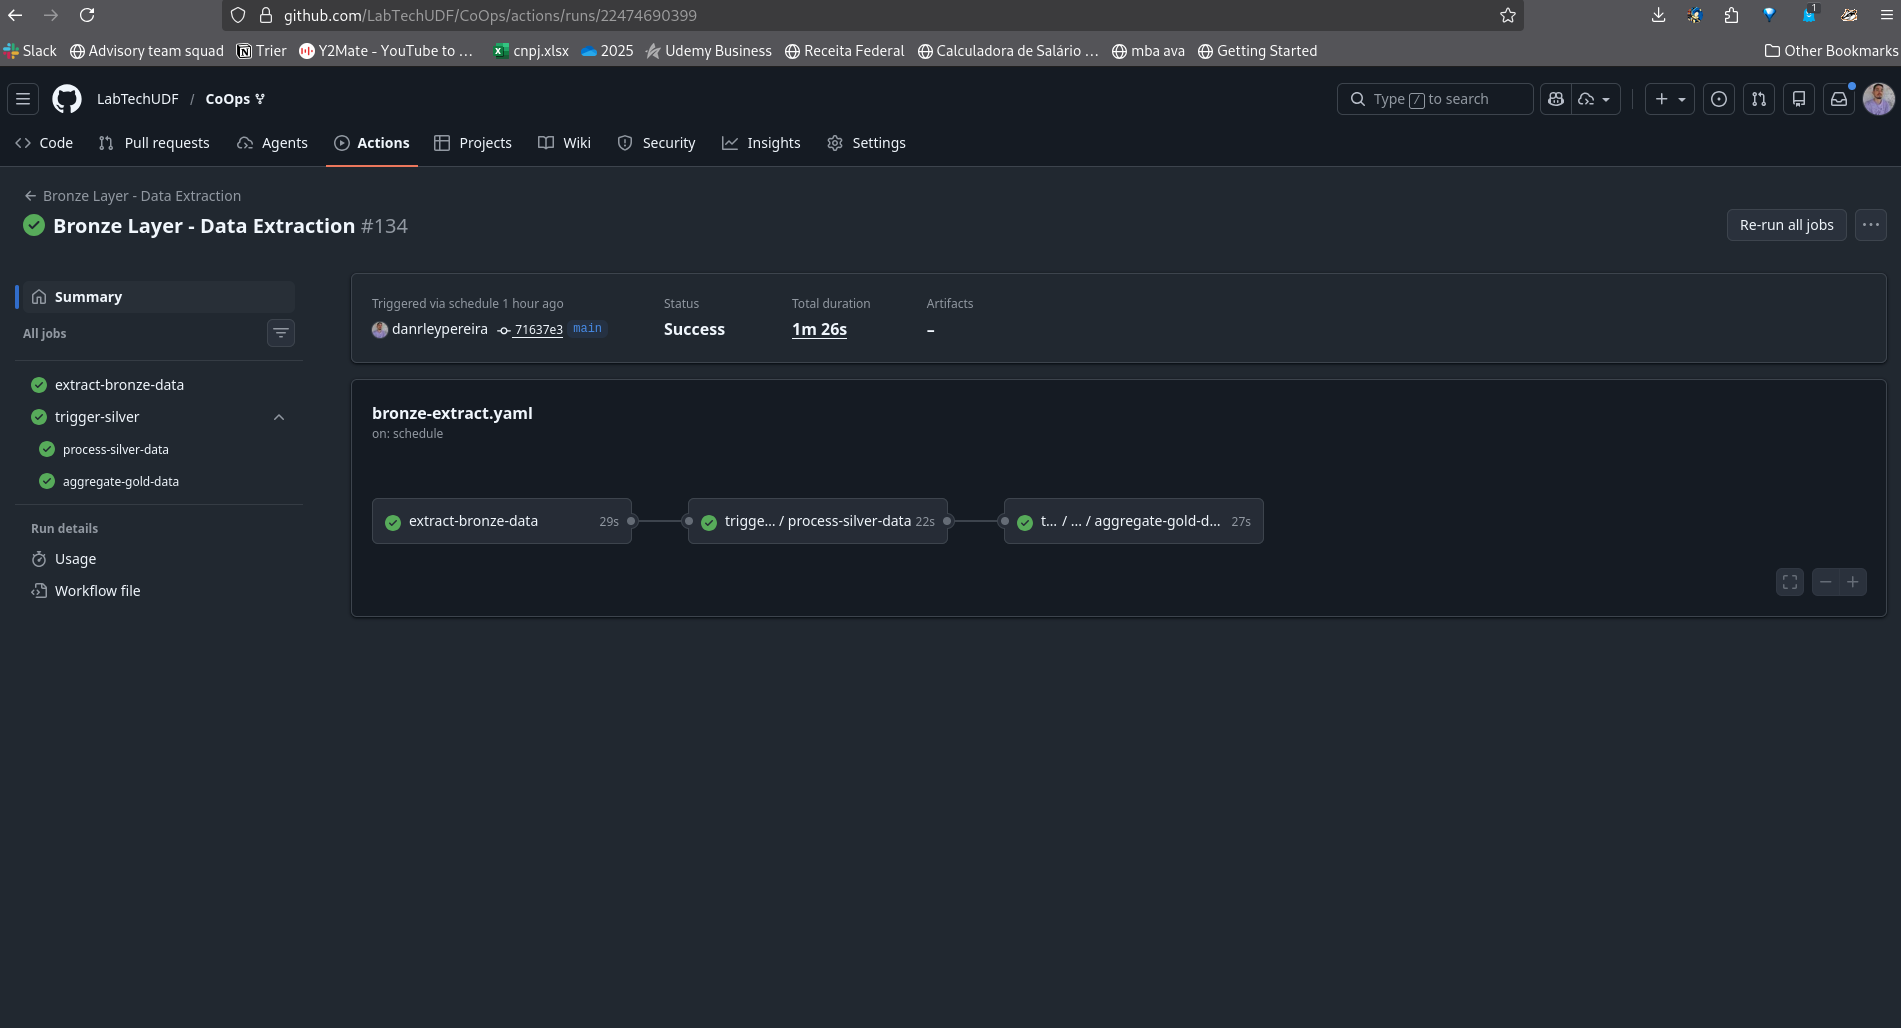
\includegraphics[width=0.9\textwidth]{screenshot-coops/pipelines-github-bronze.png}
\caption{Detalhe do pipeline Bronze no GitHub Actions.}
\end{figure}

\begin{figure}[ht]
\centering
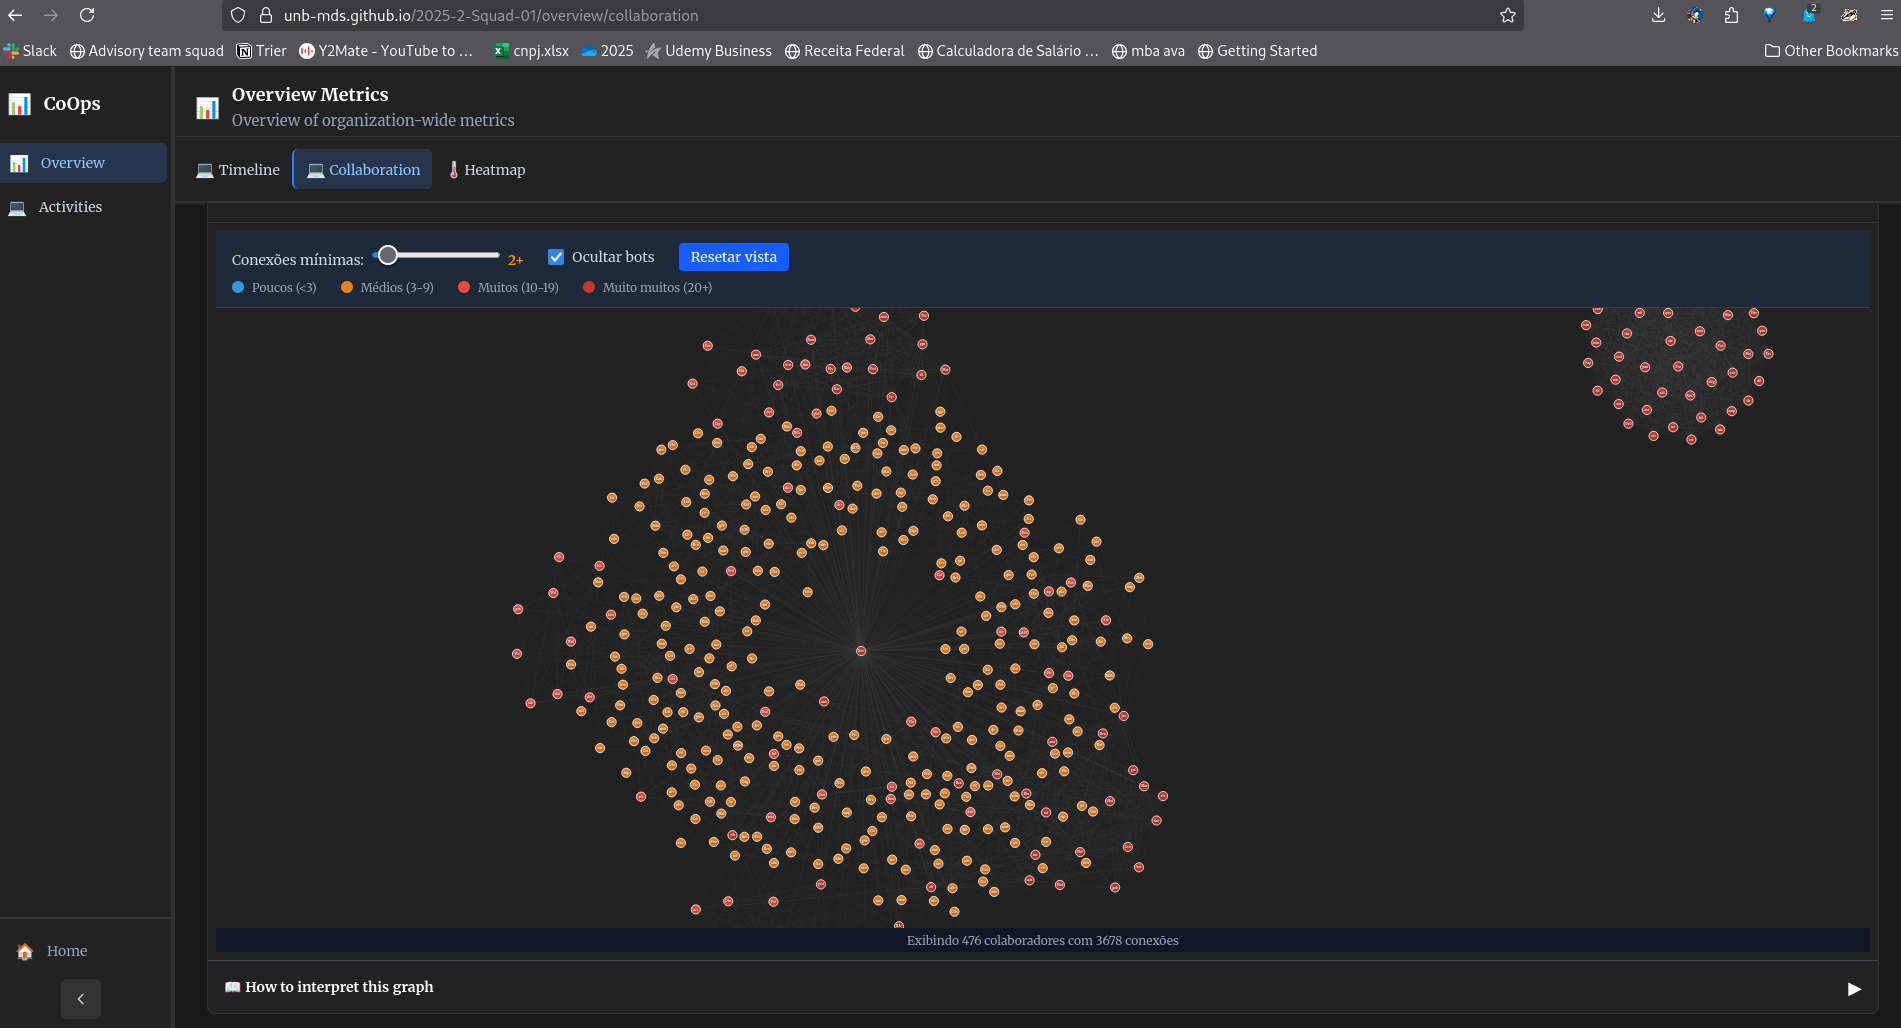
\includegraphics[width=0.9\textwidth]{screenshot-coops/rede-de-colaboracao.png}
\caption{Rede de colaboração interativa (D3.js).}
\end{figure}

\begin{figure}[ht]
\centering
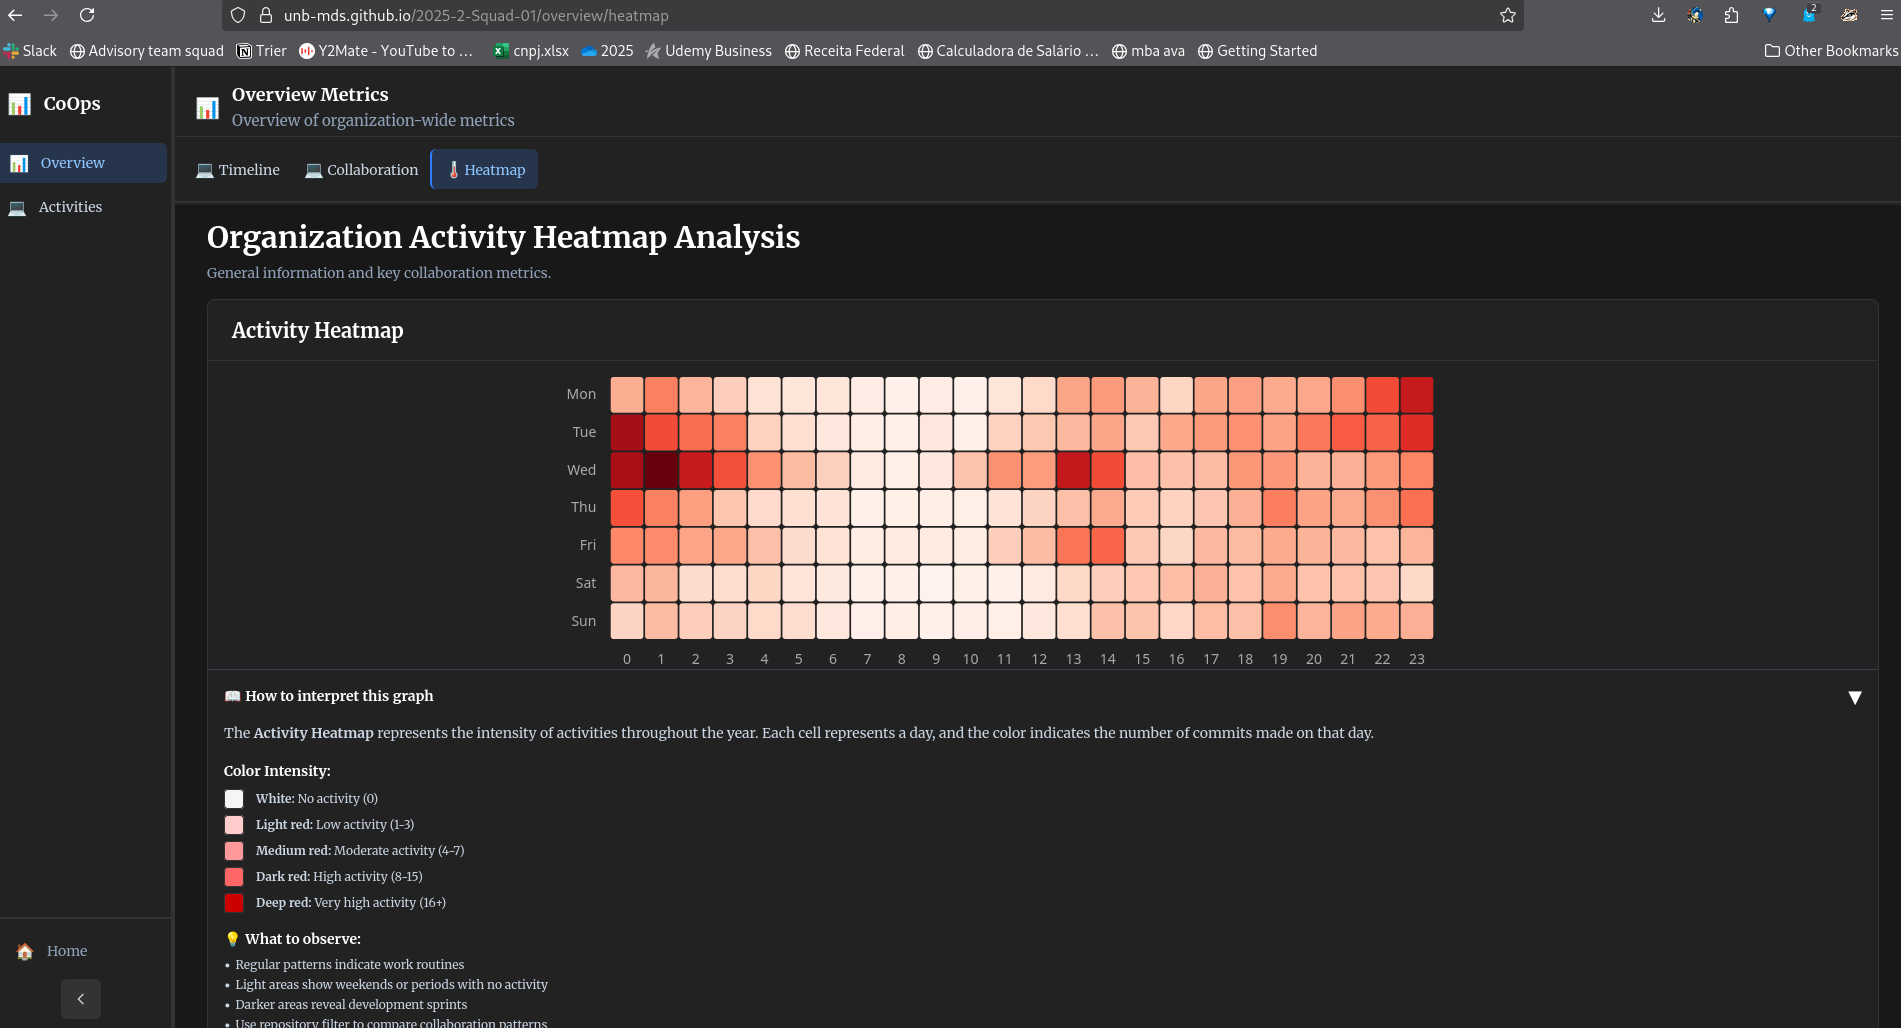
\includegraphics[width=0.9\textwidth]{screenshot-coops/heatmap.png}
\caption{Heatmap de atividade.}
\end{figure}

\begin{figure}[ht]
\centering
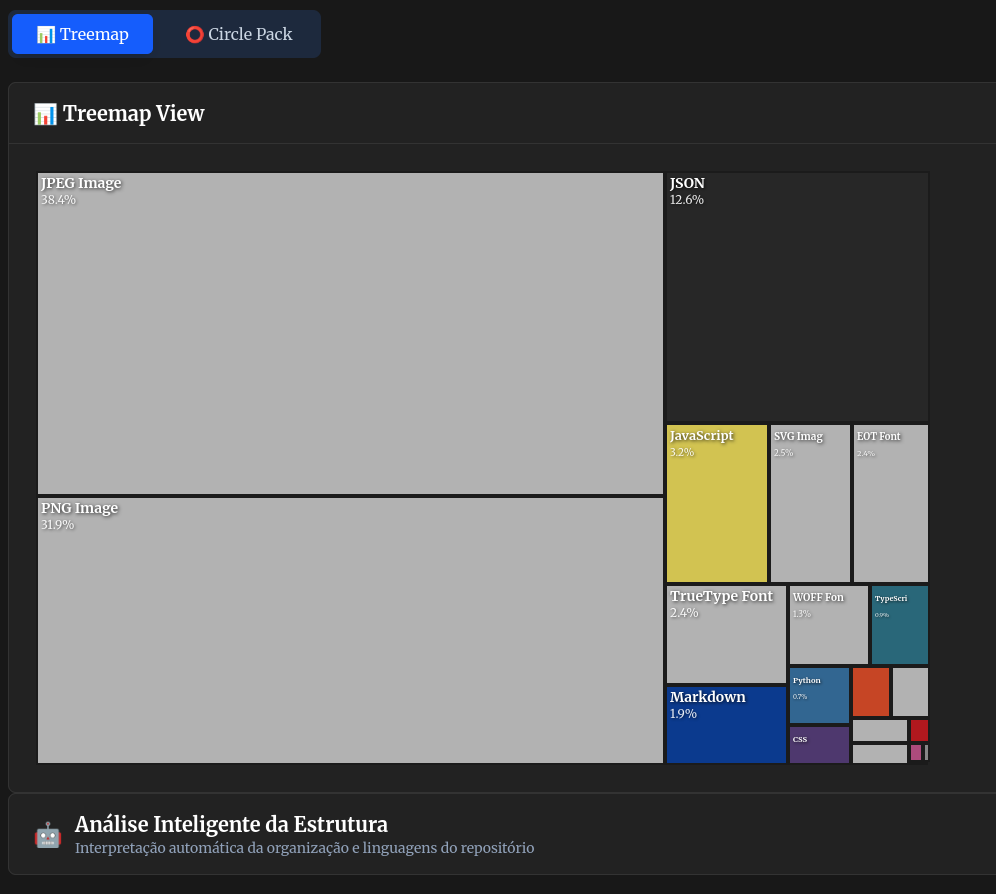
\includegraphics[width=0.9\textwidth]{screenshot-coops/treemap.png}
\caption{Visualização treemap de repositórios.}
\end{figure}

\begin{figure}[ht]
\centering
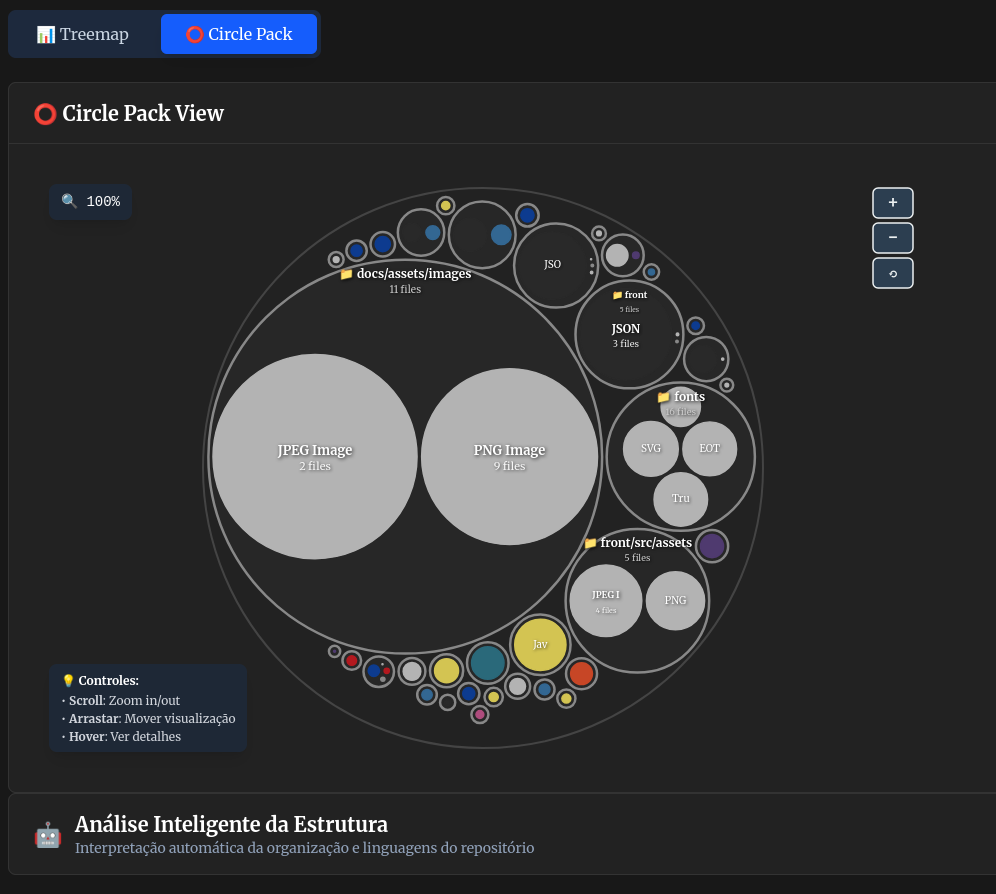
\includegraphics[width=0.9\textwidth]{screenshot-coops/circlepack-view.png}
\caption{Visualização CirclePack hierárquica.}
\end{figure}

\begin{figure}[ht]
\centering
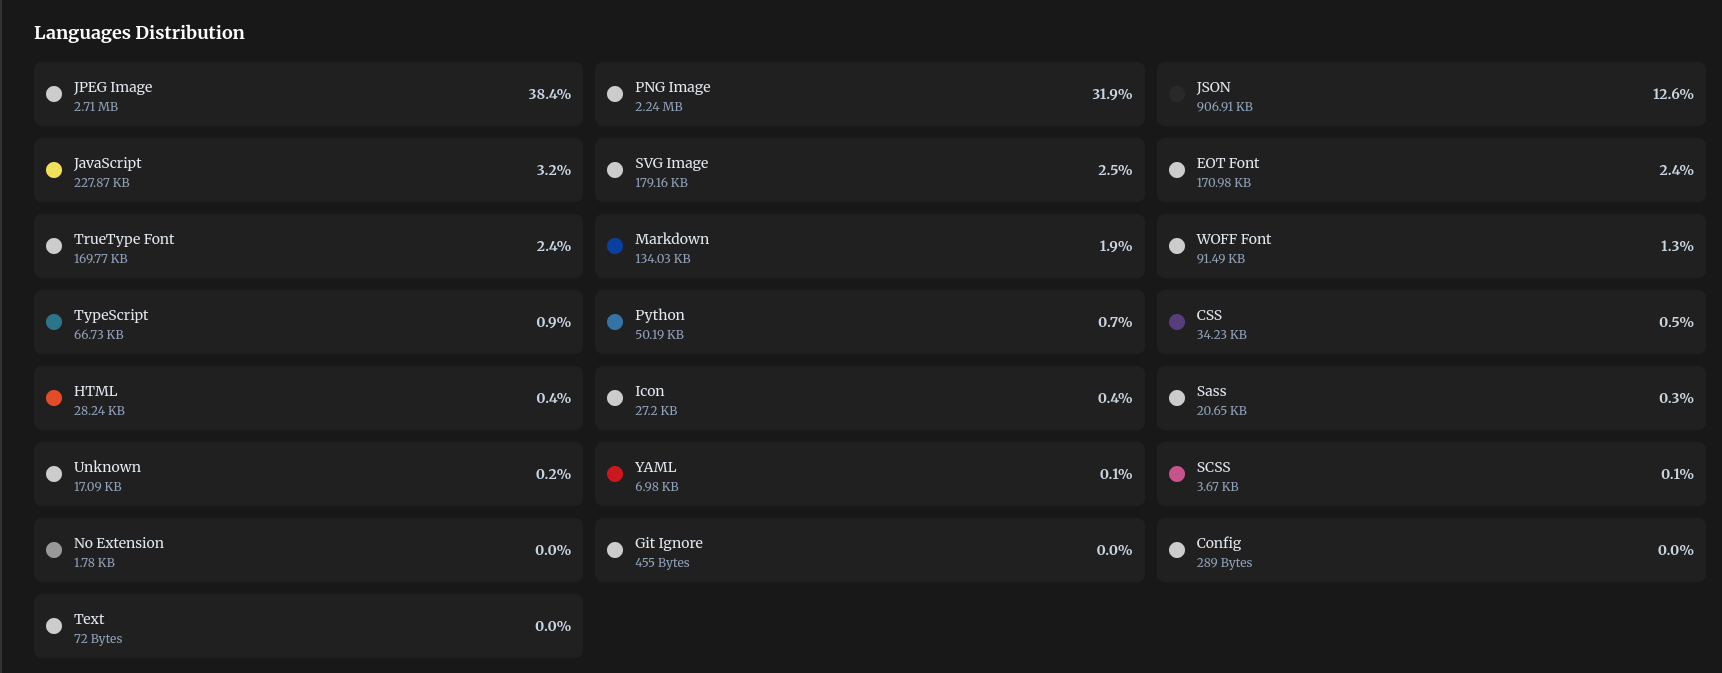
\includegraphics[width=0.9\textwidth]{screenshot-coops/language-distribution.png}
\caption{Distribuição de linguagens de programação.}
\end{figure}

\begin{figure}[ht]
\centering
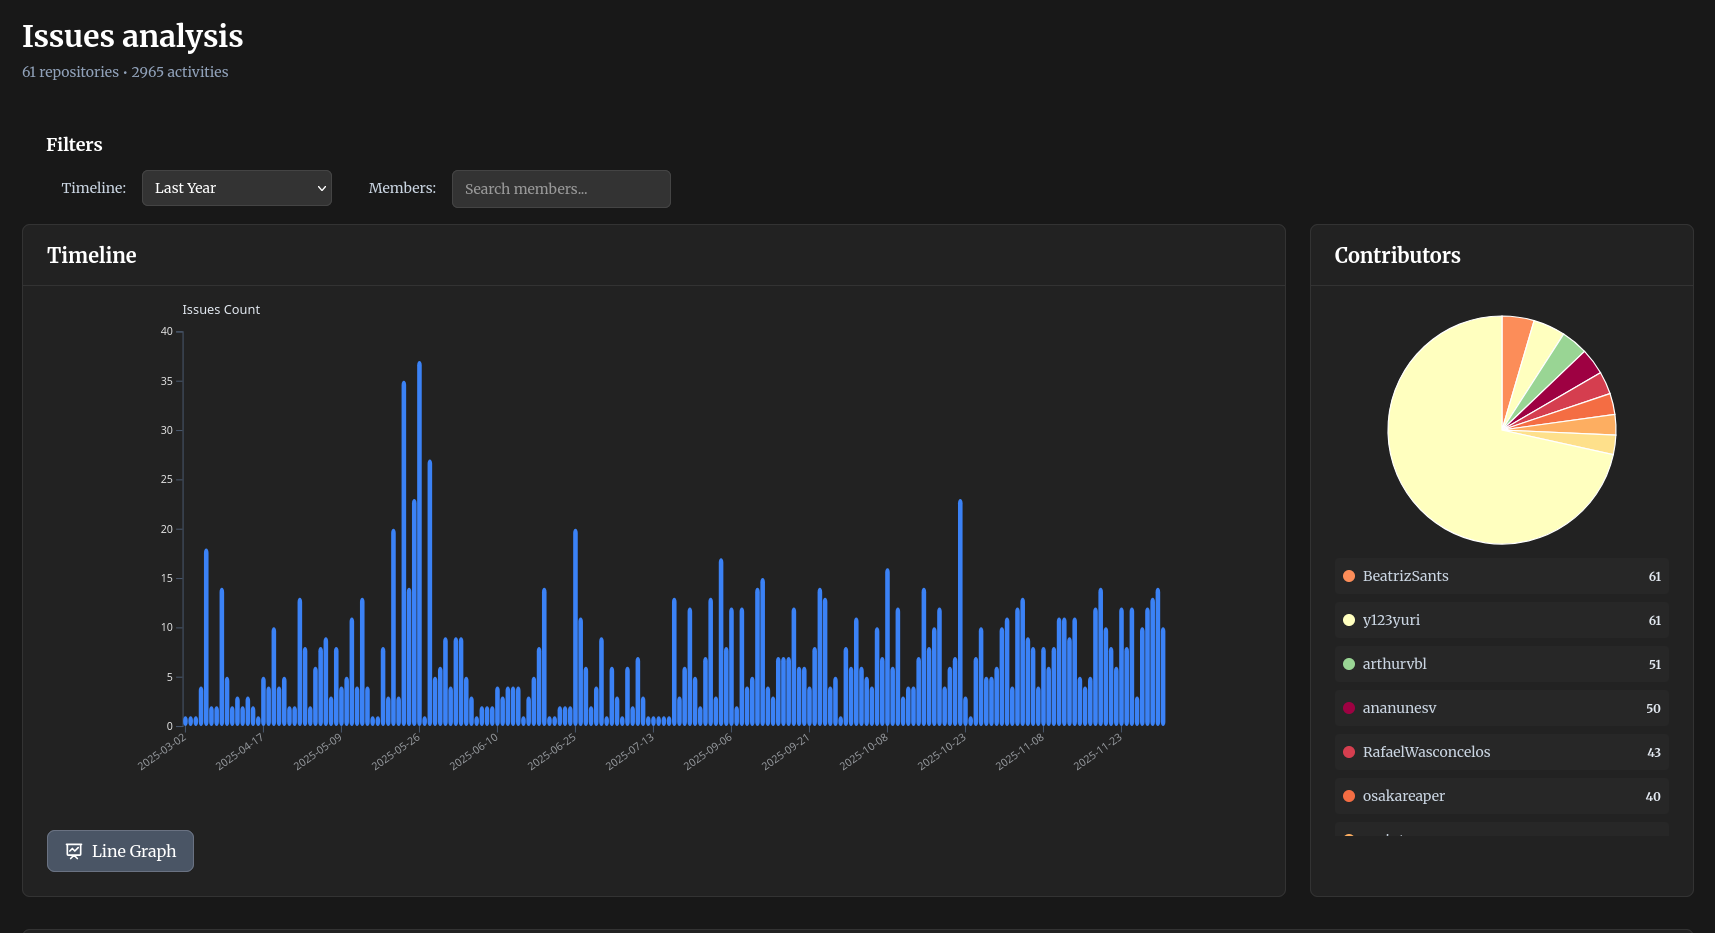
\includegraphics[width=0.9\textwidth]{screenshot-coops/issues-analysis-mds-with-contribution-pizza-graph.png}
\caption{Análise de issues com gráfico de contribuições.}
\end{figure}

\begin{figure}[ht]
\centering
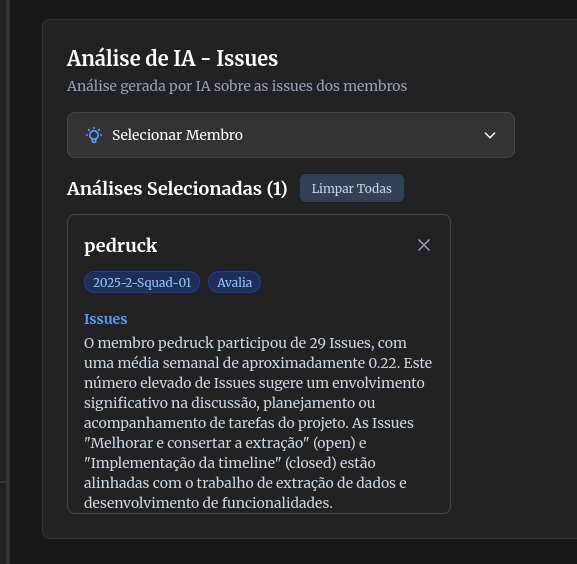
\includegraphics[width=0.9\textwidth]{screenshot-coops/ai-analysis-issues-from-one-member-from-mds.png}
\caption{Análise por IA das issues de um membro.}
\end{figure}

\begin{figure}[ht]
\centering
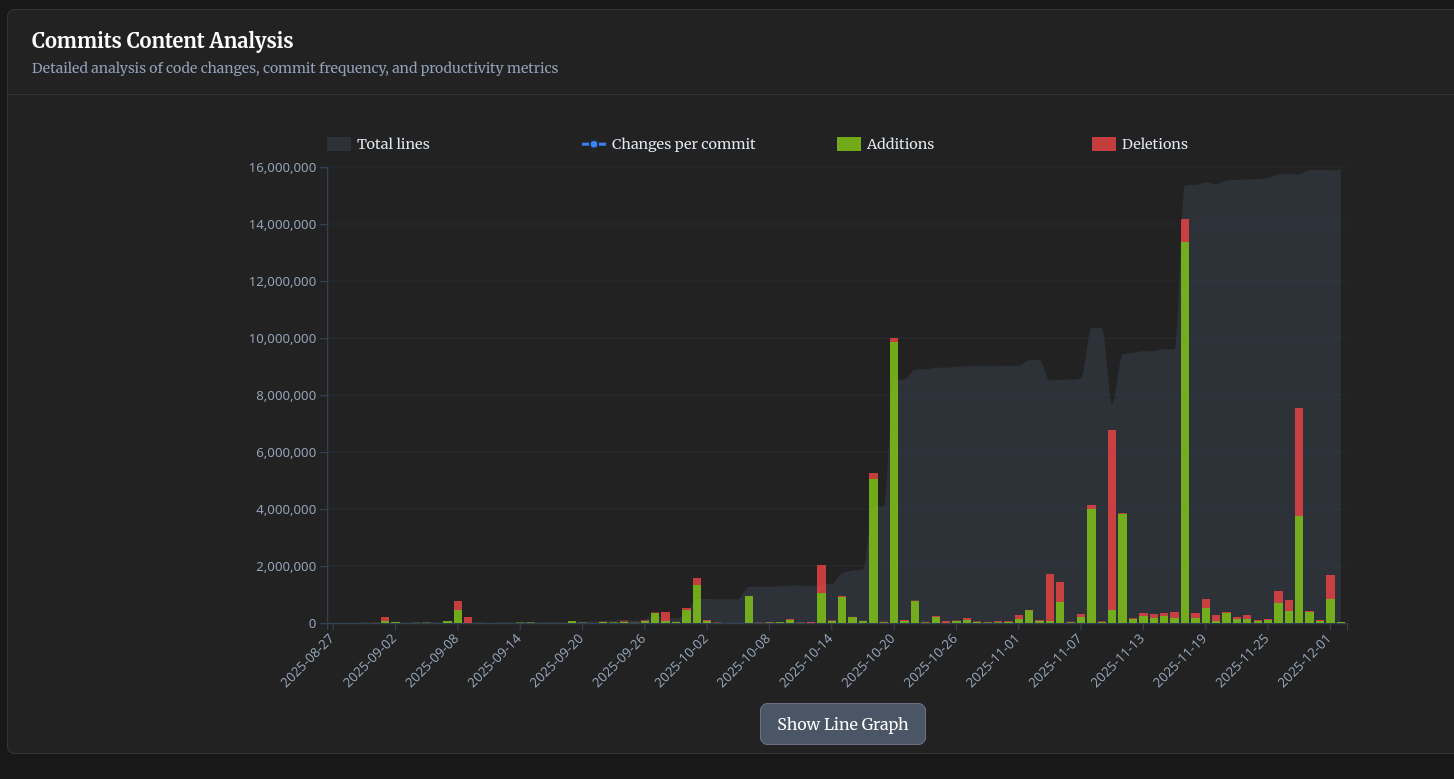
\includegraphics[width=0.9\textwidth]{screenshot-coops/commit-content-analysis-from-one-member-mds.png}
\caption{Análise de conteúdo de commits de um membro.}
\end{figure}

\begin{figure}[ht]
\centering
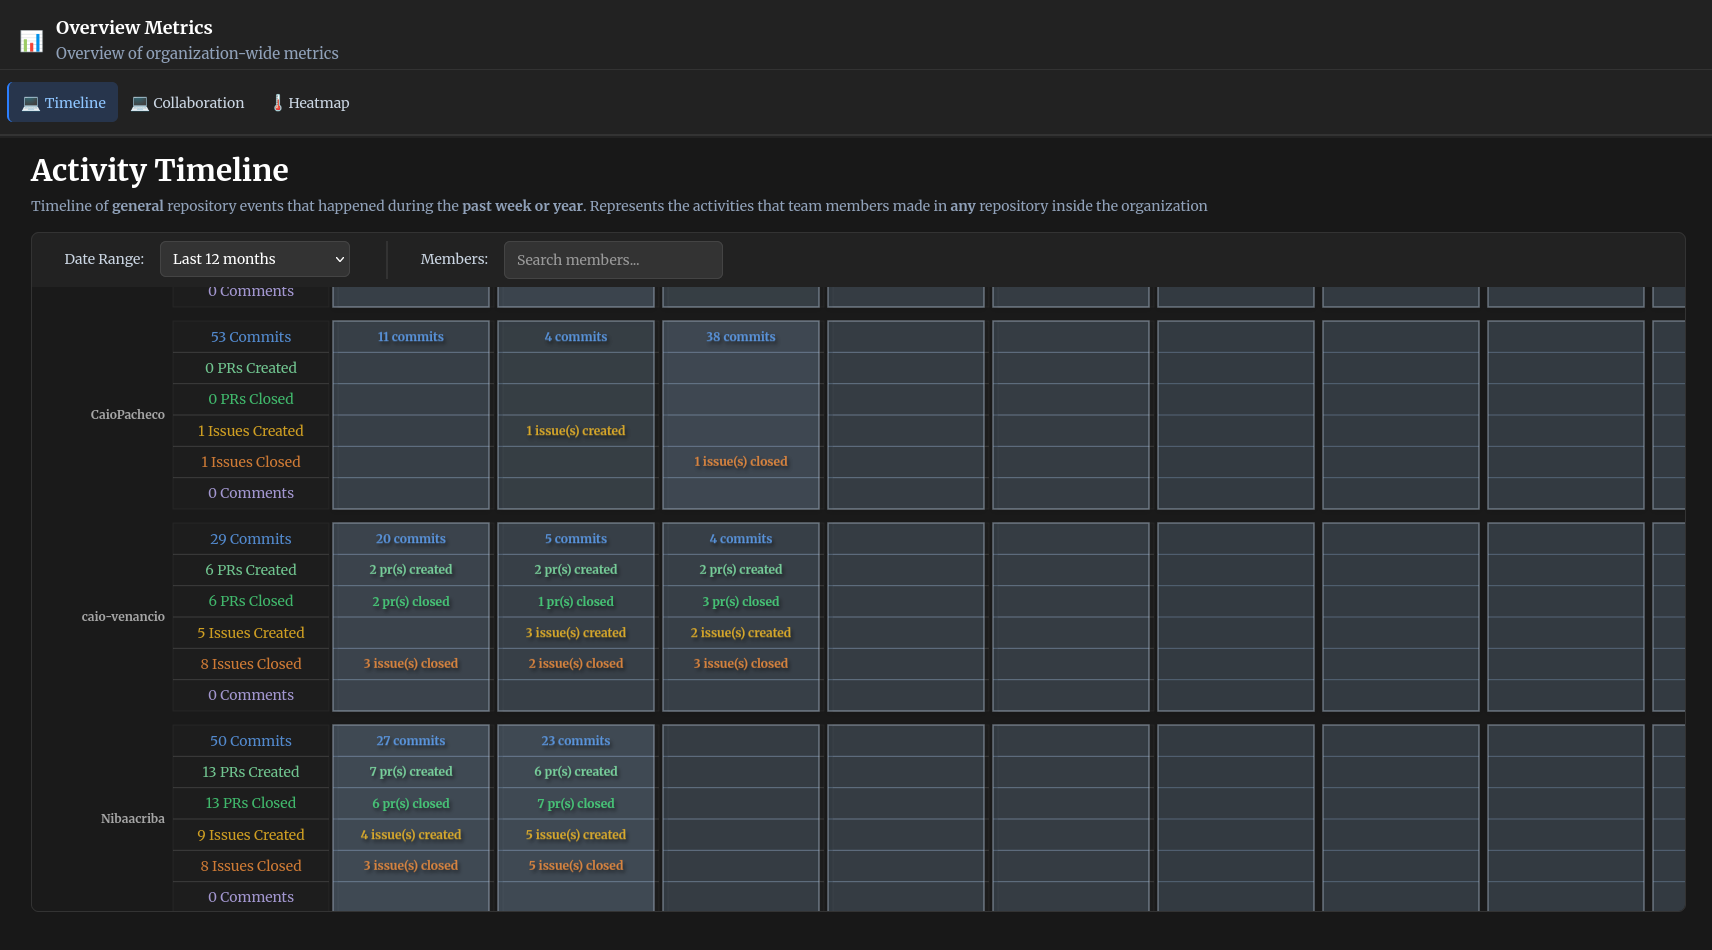
\includegraphics[width=0.9\textwidth]{screenshot-coops/activity-timeline-screen-partial-view-here-we-can-see-prs-issues-etc-by-user.png}
\caption{Timeline de atividade com PRs, issues e contribuições por membro.}
\end{figure}

\end{apendicesenv}

\end{document}
